\cleardoublepage
\chapter{Analyse og teori}
\label{chap:analysis}
\meta{
Kapittelet tar for seg analysedelen av arbeidet. Den består av to hoveddeler, en grundig beskrivelse av oppgaven basert på skissen gitt av oppdragsgiver, og en undersøkelse av hva som finnes av relatert arbeid, {\em best practise} og relevant teknologi. 
}

I dette kapittelet danner vi oss et bilde av hvordan en akademisk/teknisk rapport bør se ut, både med hensyn på innhold, struktur og utforming. Vi ser også på hvordan store og komplekse dokumenter blir produsert (både analogt og digitalt), og hva slags (digitale) verktøy som kan tenkes å brukes. Vi går også gjennom endel tilgjengelig materiale som kan gjøre det lettere å velge hva slags digitale verktøy man burde bruke i en bacheloroppgave\footnote{Utvalget er noe overfladisk utført, i hovedsak basert på forfatterens erfaringer.}.

-- 

Kapittel 2 omhandler relevant teori og beste praksis for planlegging, design og utvikling. I dette kapittelet vil vi danne oss et bilde av hvordan en nettsted bør se ut. Både med hensyn på innhold, struktur og utforming. I tillegg vil vi presentere de verktøy vi mener er passende i et slikt prosjekt.

\section{Utdypning av oppgavebeskrivelse}
Sirkus Media har gitt utrykk for at de ønsker en "one-pager". Dette vil si at nettstedet i hovedsak består av en langt nettside. Samtidig ønsker oppdragsgiver at nettstedet skal være godt synlig i Google og andre søkemotorer og at det finnes mulighet for innlogging slik at det er mulig å legge til, oppdatere og fjerne innhold. Studengruppen vil dermed utvikle et eget CMS eller benytte et ferdigutviklet system som møter disse behovene. 

CMS og API

\section{Risikoanalyse}

\section{Hvorfor et nettsted er viktig}
Å benytte seg av internett har i dagens samfunn blitt et hverdagslig gjøremål for mange. I følge undersøkelser gjort av Statistisk sentralbyrå (SSB)\footnote{Statistisk sentralbyrå utarbeider og gir ut offisiell statistikk i Norge} i 2017, hadde hele 98\% av Norges befolkning tilgang på internett hjemme \cite{ssb17fim}. Det viste seg også at 9 av 10 nordmenn surfet på nettet hver dag \cite{ssb17nat}. SSB har også kartlagt  at så mange som 89\% av Norges befolkning, mellom 16-79 år, brukte internett til å søke etter informasjon om varer eller tjenester de siste 3 måneder i 2018 \cite{ssb18aup}. Disse foregående funnene er svært relevante, og er med å underbygge hvorfor det er så viktig for en bedrift å være på internett i dag.

I tillegg til disse funnene, er det også andre faktorer som bidrar til at et nettsted for en bedrift er så viktig i dag. Disse blir presentert nærmere i dette kapittelet. 

\subsection{Treff i søk}
Når en bedrift har et nettsted blir det mulig å dukke opp i søkeresultatene hos søkemotorer\footnote{Se avsnitt \ref{sec:concepts-seo}}. I følge undersøkelser gjort av Google viser det seg at hele 76\% av de som søker på smarttelefonene etter noe i nærheten, besøker en bedrift innen en dag \cite{google16hms}. I tillegg viser undersøkelsene at når et spørsmål eller behov oppstår er sannsynligheten minst dobbelt så stor for å benytte seg av søk, enn andre online og offline kilder som sosiale medier eller å besøke butikker. Ikke bare er søk den mest brukte ressursen, det er den tjenesten 87\% vender seg til først \cite{google16mhc}. I undersøkelsene ble det også kartlagt at 51\% av brukere har oppdaget et nytt produkt eller bedrift når de har utført søk på deres telefon \cite{google16scp}. For bedrifter er det altså helt avgjørende å være godt synlig hos søkemotorer.




\subsection{Troverdighet}
\label{sec:analyse-troverdighet}
Etter studier gjort av avdelingen for informasjon og ledelse ved HuaZhong Normal University viser det seg at troverdihgeten til en bedrift sitt nettsted er en viktig faktor når brukerene skal bestemme seg for om prosessen skal gå videre eller ikke, og vil ha en stor påvirkning på deres avgjørelse når det gjelder kjøp.


\meta{The level of enterprise website credibility is an important basis for the
website browsers (or consumers) deciding whether to take
further action or not, and will have a great influence on their
purchase decision-making. }

I følge studiene kommer det også frem at kriteriene for å bestemme troverdigheten til et nettsted er basert på subjektiv vurdering og ikke profesjonell analyse. Brukere undersøker vanligvis utseende, informasjon og funksjon til nettstedet i henhold til deres faktiske behov og gjør seg deretter opp deres egen konklusjon \cite{zhao2009eew}.

\meta{As the above study shows, criterion for determining the
credibility of website is based on subjective judgment instead
of professional analysis. People usually examine the
appearance, information and function of the website
according to their actual needs and then get their own
conclusion.}
% https://ieeexplore.ieee.org/stamp/stamp.jsp?tp=&arnumber=5279898


I en studie gjennomført av BrightLocal Ltd. i 2016 ble det gjort undersøkelser på hva forbrukere ønsker fra lokale bedrifter. Resultatene ble tatt fra et panel på 800 forbrukere, der alle er basert i USA, med forskjellig alder og kjønn. Blant de 800 respondentene, var alderspennet følgende: 

\begin{itemize}
\item 18-34 – 44\%
\item 35-54 – 34\%
\item 55+ – 22\%
\end{itemize}

I denne undersøkelsen svarte 40\% av aldergruppen mellom 18-34 og 35-54 at det er mer sannsynlig at de kontakter en lokal bedrift hvis de har en nettside. På spørsmål om en klar og smart nettside øker bedriftens troverdighet, svarte 43\% av respondendene over 55 at dette hadde noe å si \cite{marchant18wdc}.

Med utgangspunktet i disse studiene kan vi derfor konkludere med at en nettside med god troverdighet kan føre til at flere potensielle kunder tar kontakt.

\subsection{Markedsføringskanal}
Nettstederer er et eksempel på et enveis nettverktøy med høy  bedrifts kontroll.
Websites and e-mail can be seen as examples of one-way online tools with high company control. https://www.emeraldinsight.com/doi/pdfplus/10.1108/JSBED-05-2013-0073. På en nettside har en bedrift altså mulighet til å bestemme innholdet og hvordan firmaet skal fremstå. Dette er en mulighet enhver bedrift burde benytte seg av, da nettstedet kan være med å forbedre og øke troverdigheten\footnote{Se avsnitt \ref{sec:analyse-troverdighet}} og dermed forholdet kunden har til bedriften.

\subsection{Innsamling av data}
En annen god grunn for å ha et nettsted, er at man kan benytte seg av verktøy som Google Analytics\footnote{Se avsnitt \ref{sec:google-analytics}}. Data samlet av Google Analytics kan brukes til å finne ut av hvilken av sidene som er mest populær eller har flest besøk. Det er også mulig å finne ut av hvilken type informasjon besøkene er interessert i, gjennom hvilken vei en bruker kommer inn og ut av siden på og hvor mye tid som har blitt brukt på nettstedet \cite{kent2011lwa}. Ved å kartlegge dette vil bedriften alltid ha oppdatert og relevant informasjon tilgjengelig, som kan brukes til å forbedre nettstedet fortløpende. 

% https://ac.els-cdn.com/S0363811111001433/1-s2.0-S0363811111001433-main.pdf?_tid=6362f9f9-b2cf-4c0f-95ac-004f5552c93e&acdnat=1550673249_e4d9b2b5340feb6427e7bd538ecd0f65


\section{Viktige faktorer innen webdesign}
Innenfor webdesign finnes det flere forskjellige faktorer er avgjørende når det kommer til hvor godt et nettsted er utført. En presentasjon av disse faktorene og hvorfor de er så viktig vil bli presentert nærmere i dette kapittelet. 

\subsection{Målgruppe}

\url{https://www.thinkwithgoogle.com/marketing-resources/tutorials/human-insights-audience-strategy/}

En målgruppe


\subsection{Design, profil og førsteinntrykk}
\url{https://www.tandfonline.com/doi/pdf/10.1080/10447318.2013.839899?needAccess=true }

\url{http://news.mst.edu/2012/02/eye-tracking_studies_show_firs/}

\url{https://www.tandfonline.com/doi/abs/10.1080/01449290500330448 }


\subsection{Responsivt design}
Undersøkelser fra Google om mobilbruk... Står om det i en av kildene som har blitt brukt tidligere

\subsection{Søkemotoroptimalisering}
\label{sec:concepts-seo}
Søkemotoroptimalisering (SEO) går ut på å oppnå gode plasseringer i de organiske søkeresulatene hos søkemotorer \cite[s.~16]{flensted10smg}. I praksis handler SEO om at en nettside blir optimalisert på en rekke områder, slik at søkemotoren finner akkurat dette nettstedet og presenterer den godt synlig i de organiske søkeresultatene ved å se på søkeordene ønsket målgruppe benytter  \cite[s.~20]{flensted10smg}.

Mer teoretisk fungerer søkemotoroptimalisering ved at de innsamlede dataene blir indeksert og lagret. Alle disse operasjonene utføres av søkemotorprogramvaren (crawler, edderkopp,
bot). Disse programmene beveger seg ved å bruke hyperkobling struktur på nettet. De navigerer regelmessig gjennom nettsider og fanger endringer som har blitt gjort siden sist  \cite[s.~488]{yalccin2010search}.

Undersøkelser viser at 75\% of Internet users never scroll past the first page of search results, TRENGER KILDE!! 
Disse funnene underbygger påstanden om at SEO er viktig i dagens samfunn, og en god SEO-strategi er derfor på sin plass. 
\url{https://www.searchenginepeople.com/blog/40-unbelievable-seo-statistics-need-know.html#note-68961-5 }

En faktor som er viktg å tenke på er at god SEO krever disiplin, planlegging og research før man setter i gang. Dette er ikke en oppgave som kun gjøres en gang, og krever konstant overvåking og optimalisering da algoritmene hele tiden endrer hvordan de evaluerer nettsider \cite[s.~1]{mitchell2012usb}. Derfor er det viktig å hele tiden ha SEO i fokus når man utvikler, når et av målene er god plassering hos søkemotorene.


\subsection{Brukeropplevelsen}
I følge Steve Krug, forfatteren bak boken \q{Don't make me think}, går brukervennlighet ut på noe så enkelt som at en helt vanlig bruker med gjennomsnittlige egenskaper og erfaring (eller til og med lavere), skal kunne finne ut av hvordan en ting skal brukes for å oppnå et mål, uten å dette fører til mer trøbbel enn det er verdt \cite[s.~9]{krug2014dmt}. Det er nettopp derfor forfatterens første lov til god brukeropplevelse er \q{ikke få meg til å tenke}. Et nettsted bør nemlig være selvforklarende, og en bruker skal intuitivt forstå hva et nettsted representerer og hvordan den kan brukes, uten å måtte anstrenge seg for å finne ut av det \cite[s.~11]{krug2014dmt}. Krug hevder at dette er viktig, fordi brukere kan tenke at det faktum at utviklerne bak dette nettstedet ikke tok seg bryet med å gjøre ting åpenbart og enkelt, vil påvirke deres inntrykk av siden og hele bedriften bak den \cite[s.~15]{krug2014dmt}.

\url{https://www.thinkwithgoogle.com/marketing-resources/experience-design/strong-audience-design/}

\subsubsection{Hastighet}

Bouncerate 
\url{https://www.section.io/blog/page-load-time-bounce-rate/ }


\section{Lovverk}
Det finnes også noen lovverk som må følges når det kommer til utvikling av nettsteder. I dette underkapittelet blir det beskrevet hva disse går ut på. Det blir også gjennomgått hvorfor disse lovene er viktig, utover det faktum at de er lovpålagt. 

\subsection{WCAG 2.0}

\subsection{GDPR}



\section{Beste praksis og tidligere undersøkelser}
Undersøkelser viser at følgende struktur på en nettside er å foretrekke...:

Finne et nettsted som følger best practice og skrive om det.

Obvious Always Wins:
\url{https://www.lukew.com/ff/entry.asp?1945}

\subsection{Innhold}
https://www.brightlocal.com/2016/03/04/gender-age-what-consumers-want-from-local-business-websites/ 
\subsection{Struktur}

\subsection{Sikkerhet}
 (hashing av passord. sende data over kryptert kanal)

\section{Analyse av opprinnelig løsning}

Målet med å analysere det nåværende nettstedet til Sirkus Media er å kartlegge eventuelle problemerområder som burde forbedres. Når utviklingen av det nye nettstedet er ferdig vil vi sammenligne de nye testresultatene med resultatene som blir presentert i dette kapittelet.
Se figur \ref{fig:analysis-current-sirkusmedia.no} for bilde av nettsiden på PC og mobil.

\begin{figure}[H]
    \begin{center}
        \subfigure[PC]{
            \label{fig:analysis-current-sirkusmedia.no-desktop}
            \frame{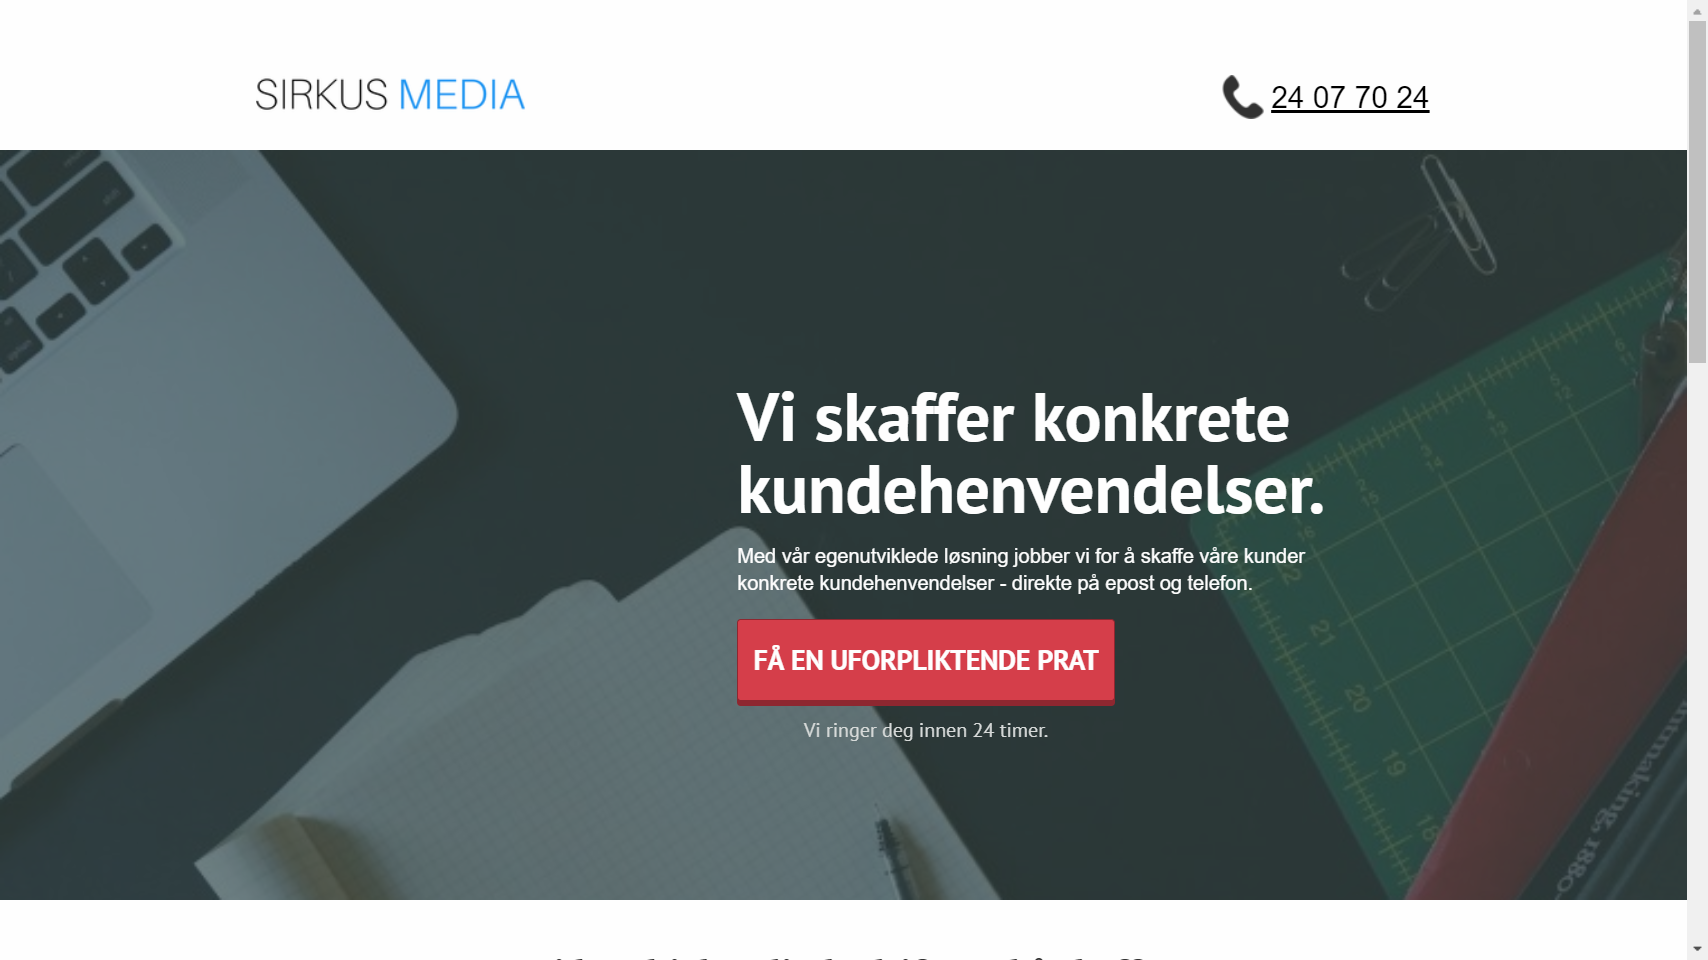
\includegraphics[width=0.7\textwidth]{bjornar/sirkusmedia_no_(1366x768).png}}
        }
        \subfigure[Mobil]{
            \label{fig:analysis-current-sirkusmedia.no-mobile}
            \frame{
\includegraphics[width=0.25\textwidth]{bjornar/sirkusmedia_no_(iPhone_6_7_8).png}}
        }
        \label{fig:analysis-current-sirkusmedia.no}
        \caption{sirkusmedia.no}
    \end{center}
\end{figure}

\subsection{Test med Google Chrome DevTools}
Google Chrome DevTools\footnote{\url{https://developers.google.com/web/tools/chrome-devtools/}} er et utviklerverktøy som følger med nettleseren Google Chrome. Det lar oss blant annet sjekke hastighet og kontrastforhold på siden og kjøre tester med Google Lighthouse.

Vi testet hastigheten til siden på det trådløse nettverket til Høgskolen i Østfold (avdeling Halden) fra en Dell XPS 13 (9350).
Resultatene måles i millisekunder.

\begin{table}[H]
\begin{tabular}{lllll}
Test & DOM & Load &  &  \\
1 & 268 & 624 &  &  \\
2 & 203 & 550 &  &  \\
3 & 216 & 560 &  &  \\
4 & 387 & 928 &  &  \\
5 & 210 & 572 &  &  \\
6 & 634 & 844 &  &  \\
7 & 309 & 857 &  &  \\
8 & 256 & 670 &  &  \\
9 & 348 & 673 &  &  \\
10 & 249 & 579 &  &  \\
\end{tabular}
\end{table}

Gjennomsnitt:\\
- DOM: 308ms\\
- Load: 614ms

Innlastningstiden til DOM beskriver hvor lang tid det tar for nettleseren å lese gjennom og analysere HTML-koden til nettsiden. Load vil si hvor lang tid det tar å laste inn DOM sammen med alle bilder, stylesheets, scripts og iframes.

\subsection{Test med Google Lighthouse}
\label{sec:analysis-current-lighthouse}

Ved å kjøre Google Lighthouse får vi resultater for hastighet, tilgjengelighet, beste praksis, søkemotoroptimalisering og progressiv webapplikasjon. Figur \ref{fig:analysis-current-lightouse-summary} viser oppsummering av resultatetene etter å ha kjørt testen. Oversikten viser at nettstedet får gode poengsummer på alle områdene. Hovedgrunnen til dette er at dagens nettsted består av kun en forside og lite informasjon. Dette begrenser muligheten for feil.

\begin{figure}[H]
    \centering
    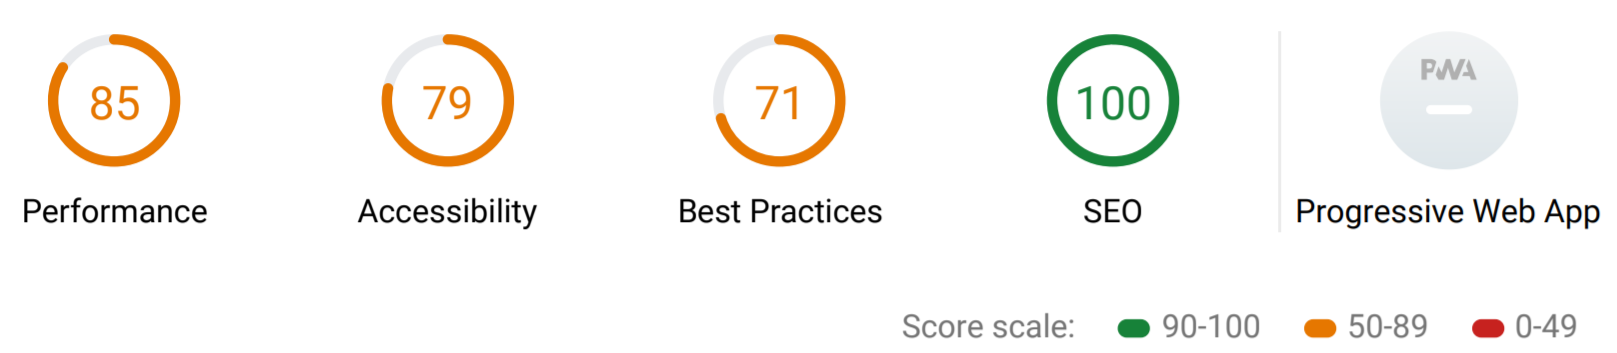
\includegraphics[width=\textwidth]{bjornar/Lighthouse-Report-mobile.png}
    \caption{Resultater fra Google Lighthouse}
    \label{fig:analysis-current-lightouse-summary}
\end{figure}

Ikonet for \q{Progressive Web App} har en feil, slik at man ikke får sett scoren. Ved hjelp av en JSON-fil\footnote{Se JSON-fil, linje 3386} som inneholder resultatene, ser man at poengscoren er på 58\%.

Denne delen av testen er egentlig ikke relevant\footnote{Sirkus Media sitt nettsted er ikke, og kommer ikke til å bli en progressiv webapplikasjon. KILDE OM PWA}, og vi vil derfor ikke se på denne, eller nevne den i andre tekniske analysener som bruker Google Lighthouse.

I rapporten kan vi se at Google laster inn nettsiden på 2,7 sekunder og at det tar 4,9 sekunder før siden blir beregnet som interaktiv. Hovedproblemet til siden er bruken av \q{render-blocking resources}\footnote{Hva er dette?}. Dette kan lett fikses og kan i følge Google spare 1,34 sekunder. Google påpeker også at det finnes 3 sikkerhetshull i JavaScript-biblioteker som blir brukt på nettsiden. Dette er ikke ønskelig, da dette øker risikoen for uønskede hendelser.

Full rapport for Google Lighthouse testen kan leses i vedlegg X.

\subsection{Checkbot}
\begin{figure}[H]
    \centering
    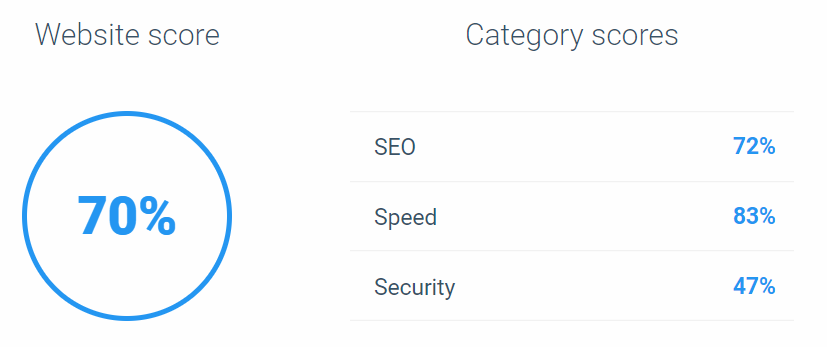
\includegraphics[width=0.75\textwidth]{bjornar/checkbotio-summary.png}
    \caption{Checkbot.io summary}
    \label{fig:analysis-current-checkbot-summary}
\end{figure}

Checkbot\footnote{https://checkbot.io} tester sikkerhet, hurtighet og søkemotoroptimalisering. Figur \ref{fig:analysis-current-checkbot-summary} viser oppsummering av resultatene. En mer detaljert rapport kan leses under vedlegg X. Denne testen viser en god poengsum når det gjelder totalt for gjennomsnittet. Isolert sett ser vi at sikkerheten til nettstedet drar ned gjennomsnittet betydlig. Den fulle rapporten viser at dette kommer av at nettsiden ikke bruker HSTS, \q{content sniffing protection}, \q{clickjack protection}, \q{XSS protection} og at det ikke skjuler server-versjon data.

\subsection{Color Contrast Analyzer}
\label{sec:analysis-current-color-contrast-analyzer}
Color Contrast Analyzer\footnote{\url{https://accessibility.oit.ncsu.edu/tools/color-contrast-chrome/}} tar bilde av nettstedet og scanner deretter kontrasten. Områder med bedre kontrast utheves og får lyse kanter. Jo mer markante kanter, desto mer kontrast.

\begin{figure}[H]
    \centering
    \makebox[\textwidth]{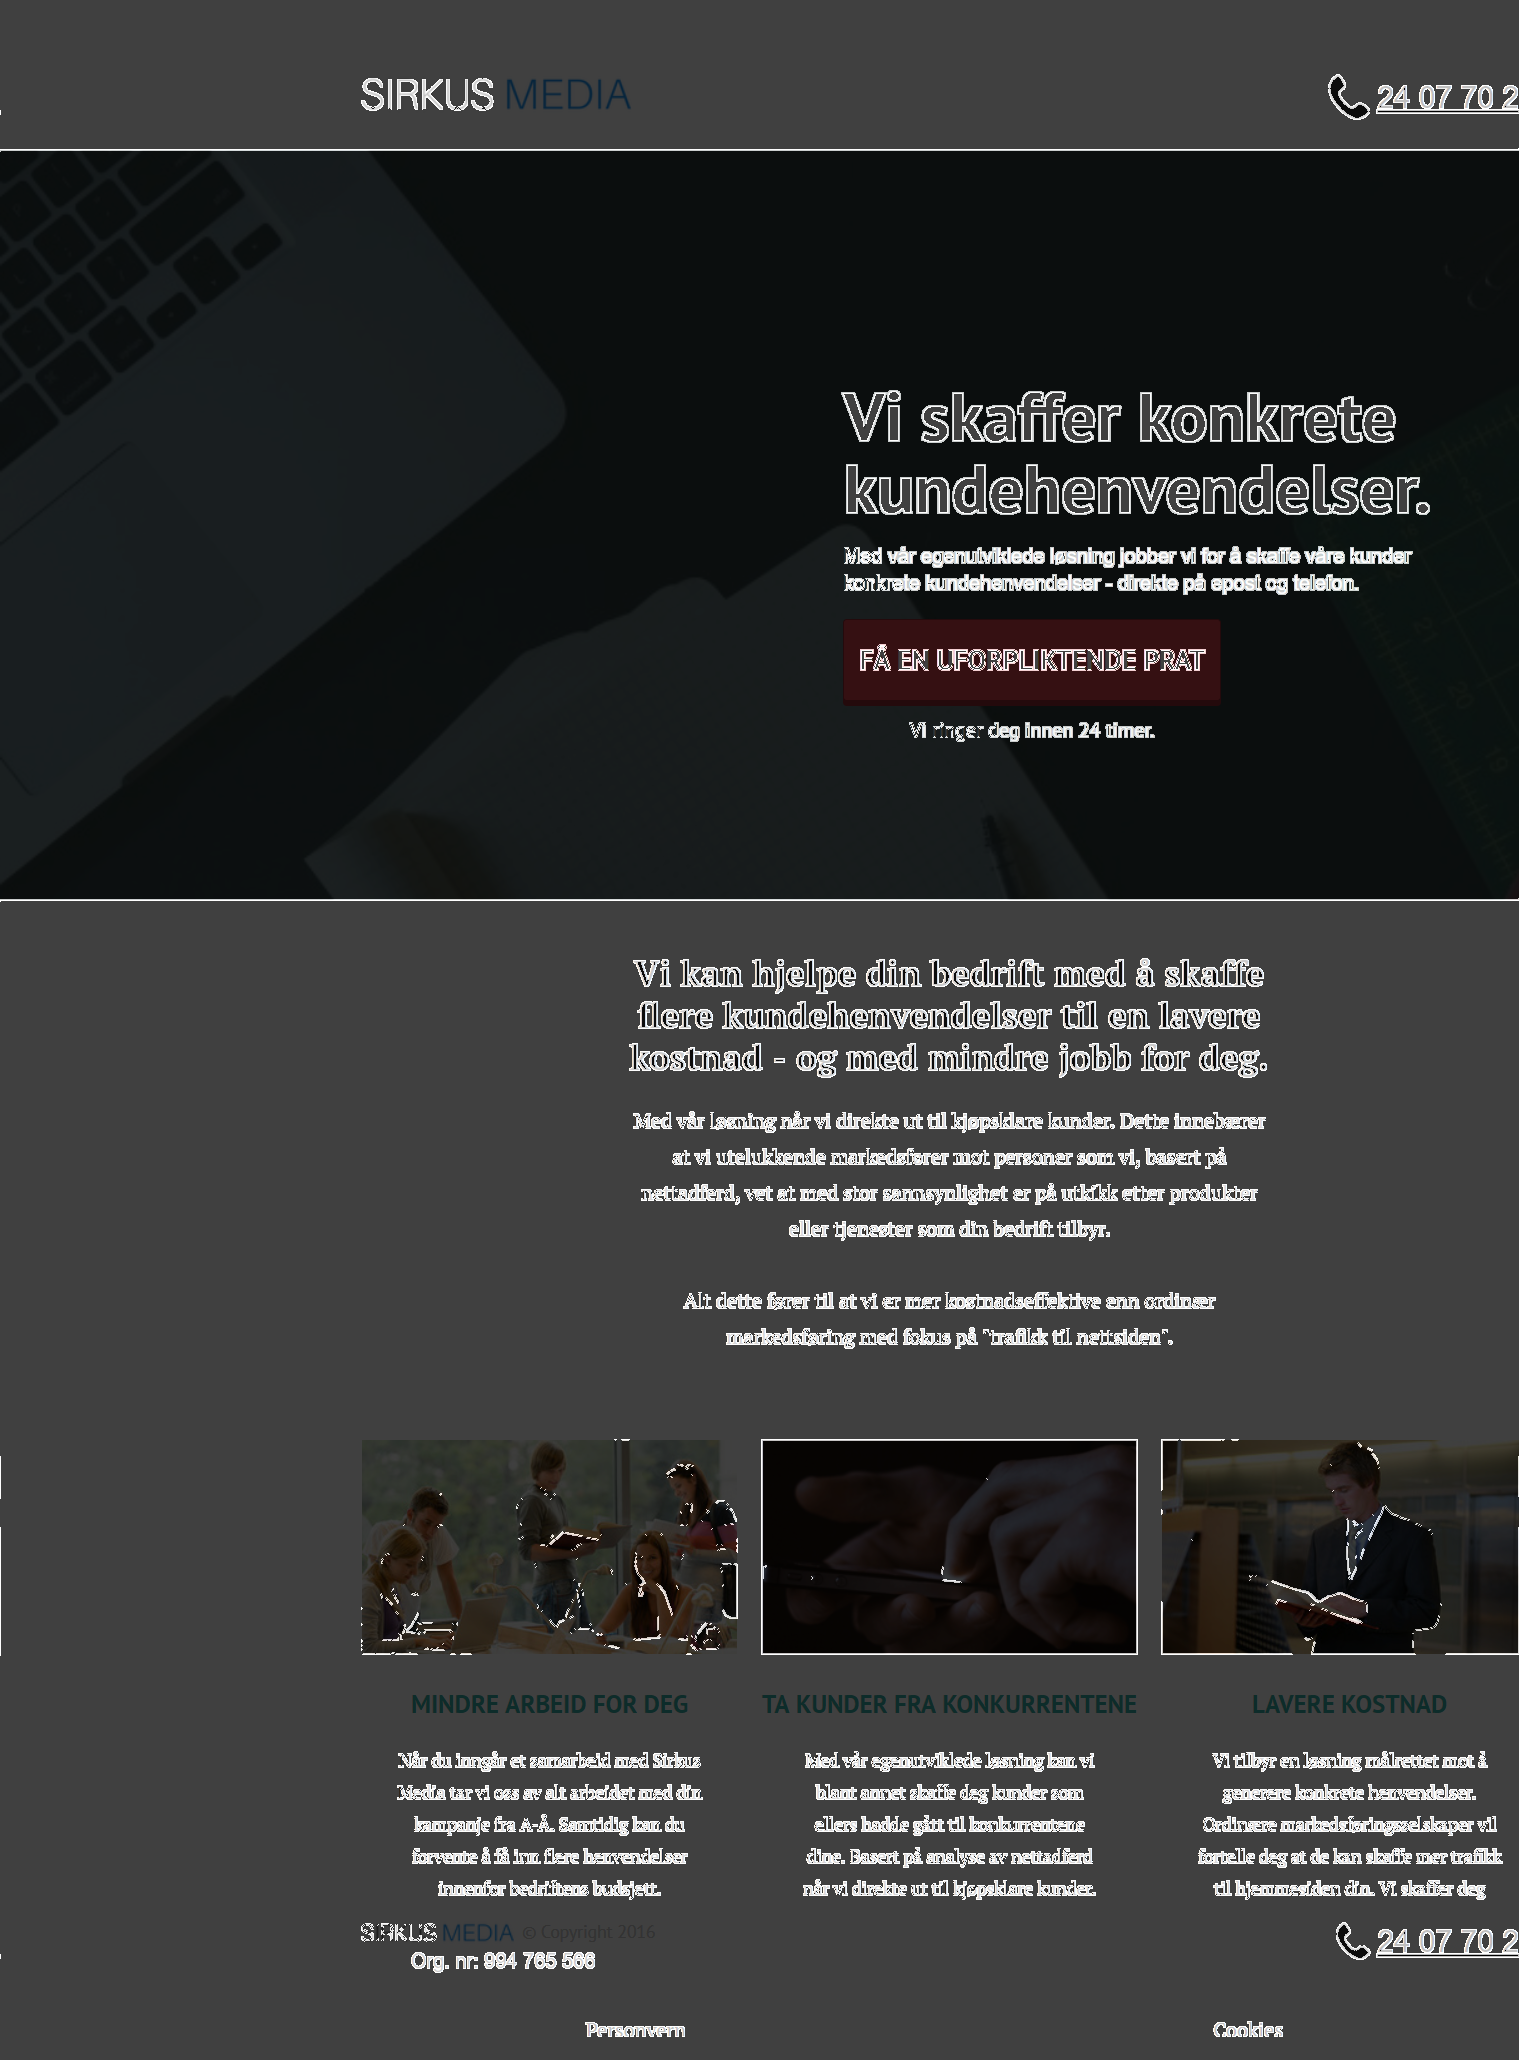
\includegraphics[width=0.80\paperwidth]{bjornar/contrast-wcag-aa-small.png}}
    \caption{CCA resultat AA}
    \label{fig:analysis-current-cca-aa}
\end{figure}

\begin{figure}[H]
    \centering
    \makebox[\textwidth]{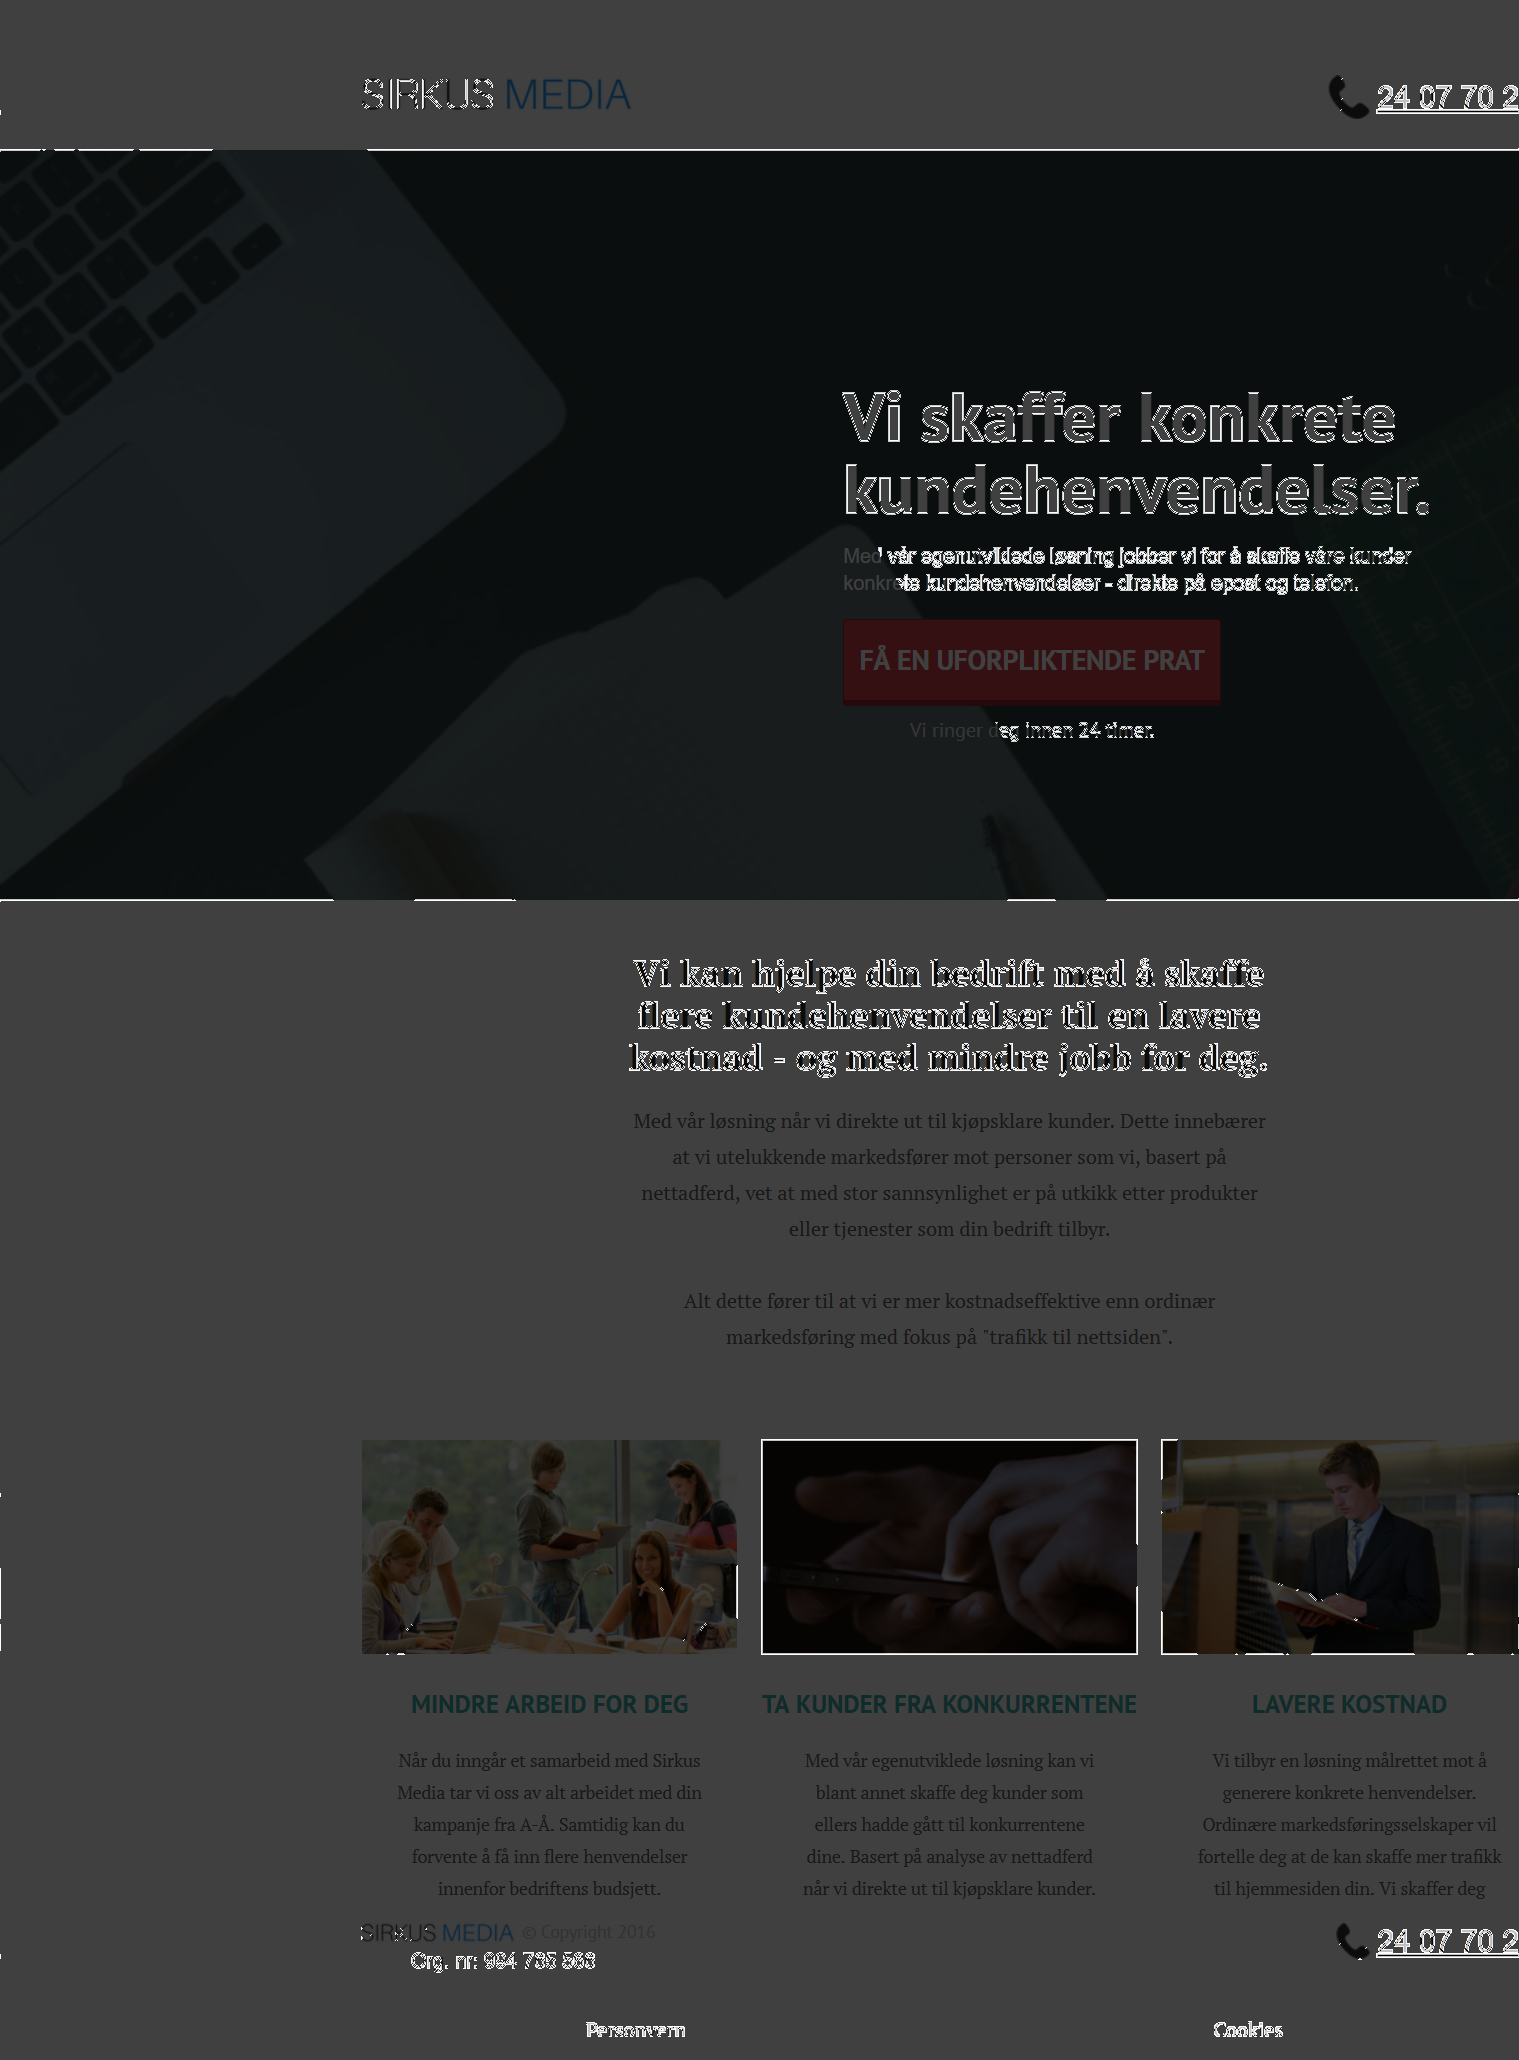
\includegraphics[width=0.80\paperwidth]{bjornar/contrast-wcag-aaa-small.png}}
    \caption{CCA resultat AAA}
    \label{fig:analysis-current-cca-aaa}
\end{figure}

Ved å kjøre testen \q{small non bold text} for nivå AA, som gjelder for skriftstørrelser opptil 18pt, viser resultatene at deler av teksten i logo og de grønne overskriftene ikke har gode nok kontraster. Dette illustreres i figur \ref{fig:analysis-current-cca-aa}. Google Chrome DevTools verifiserer at kontrastforholdet ikke oppfyller kontrastkravet for AA. Se figur \ref{fig:analysis-current-cdt-a} og \ref{fig:analysis-current-cdt-b}

\begin{figure}[H]
    \begin{center}
        \subfigure[grønn overskrift]{\label{fig:analysis-current-cdt-a}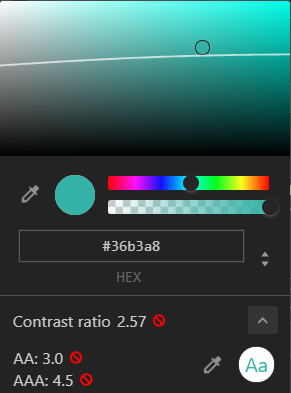
\includegraphics[width=0.3\textwidth]{bjornar/contrast-wcag-aa-small-gronn-tekst.png}}
        \subfigure[blå tekst i logo]{\label{fig:analysis-current-cdt-b}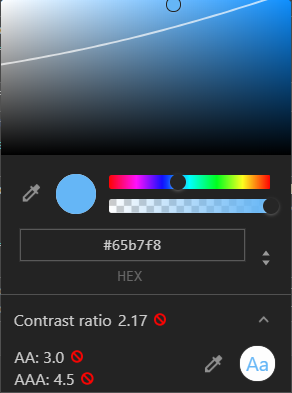
\includegraphics[width=0.3\textwidth]{bjornar/contrast-wcag-aa-small-logo-blaa.png}}
        \subfigure[vanlig tekst]{\label{fig:analysis-current-cdt-c}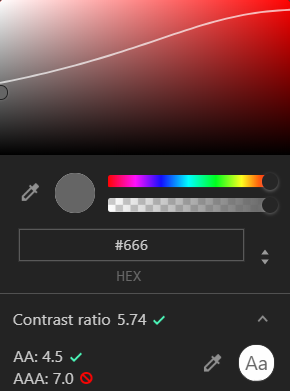
\includegraphics[width=0.3\textwidth]{bjornar/contrast-wcag-aaa-small-body.png}}
        \caption{Google Chrome DevTools - kontrastforhold}
        \label{fig:analysis-current-cdt}
    \end{center}
\end{figure}

Resultatene etter å ha kjørt tester for nivå AAA viser at mesteparten av nettstedet ikke oppfyller kravet for kontrastnivå. Se figur \ref{fig:analysis-current-cca-aaa}. Her blir ingen av avsnittene med ordinær skriftstørrelse markert. Ved å kjøre en test med Chrome DevTools verifiseres påstanden om for dårlig kontrastnivå. Se figur \ref{fig:analysis-current-cdt-c}.

\subsection{WAVE}
Med verktøyet WAVE\footnote{\url{http://wave.webaim.org/}} kan vi videre verifisere funnene som ble gjort i avsnitt \ref{sec:analysis-current-color-contrast-analyzer}. WAVE raporterer om 20 kontrastfeil på nettsiden. \vskip 1em Det ble også oppdaget andre feil:\\ \quad 1x: Dokument språk mangler\\
\quad 4x: Tomme linker\\
\quad 5x: Redudante linker\\
\vskip 1em Annet:\\
\quad 8x: Bilder med tom alt-attributt.\\
\vskip 1em Ved å skru på \q{No-styling} vil man oppdage at det er en skjult seksjon på siden (\q{THE COMPANIES THAT MAKE THEIR LIFE SIMPLE}). Dette blir plukket opp av noen skjermlesere og er derfor ikke ideelt.\\
WAVE viser også at nettstedet har bra stuktur på overskrifter og følger beste praksis.

\subsection{Kontrastforhold mellom tekst og bakgrunnsbilder}
Etter å ha testet kontrasten til siden med verktøyet fra avsnitt \ref{sec:analysis-current-color-contrast-analyzer} og Google Chrome DevTools, vet vi enda ikke om kontrastforholdet i headeren er bra nok. Vi kan se på figur \ref{fig:analysis-current-cca-aa} og \ref{fig:analysis-current-cca-aaa} at det teksten i headeren blir uthevet, og er noe svakere i figur \ref{fig:analysis-current-cca-aaa} enn i \ref{fig:analysis-current-cca-aa}. Dette må vi undersøke nærmere.

Dette er ikke mulig å sjekke med Chrome DevTools eller WAVE. Begge verktøyene vil gi negative resultater som ikke stemmer ettersom de ikke får en bakgrunnsfarge å se på, men et bakgrunnsbilde. Dette fører til at testen ikke blir utført korrekt.

For å løse dette bruker vi Brandwood sin A11y-test\footnote{\url{https://www.brandwood.com/a11y/}}. Verktøyet deler opp bilde i seksjoner og finner gjennomsnittsfargen i hver av disse seksjonene. Deretter sjekkes kontrastforholdet mellom teksten sin farge og fargen i de seksjonene som teksten er over. I figur \ref{fig:analysis-current-a11y_bg-example} kan man se eksempel på resultatet av en test. Her testet vi en hvit tekst mot et bilde av en regnbue. 

\begin{figure}[H]
    \centering
    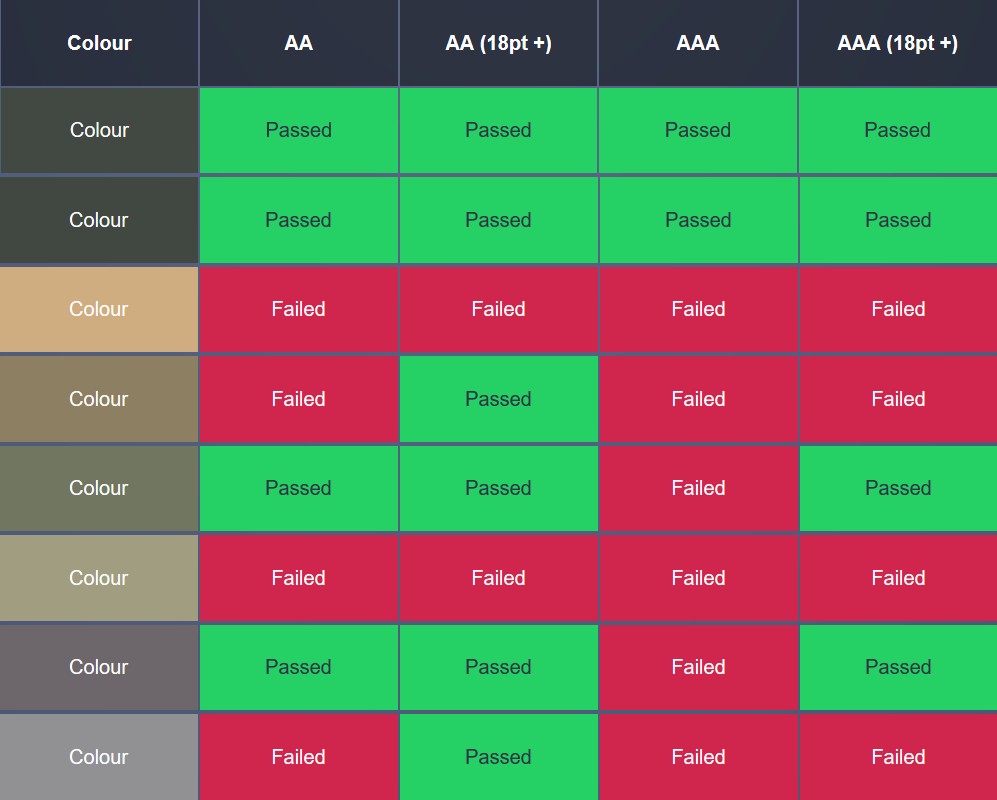
\includegraphics[width=\textwidth]{bjornar/bg-image-eksempel.png}
    \caption{Eksempel}
    \label{fig:analysis-current-a11y_bg-example}
\end{figure}

Vi gjenskapte headeren til Sirkus Media i verktøyet, og testet den store teksten: \q{Vi skaffer konkrete kundehenvendelser} og den mindre teksten \q{Med vår egenutviklede løsning jobber vi for å skaffe våre kunder konkrete kundehenvendelser - direkte på epost og telefon.} Se figur \ref{fig:analysis-current-a11y_bg-generator}. 

\begin{figure}[H]
    \centering
    
\includegraphics[width=\textwidth]{bjornar/bg-image-generator.png}
    \caption{Stor tekst fra header i verktøyet}
    \label{fig:analysis-current-a11y_bg-generator}
\end{figure}

\begin{figure}[H]
    \begin{center}
        \subfigure[Stor tekst]{\label{fig:analysis-current-a11y_bg-h1}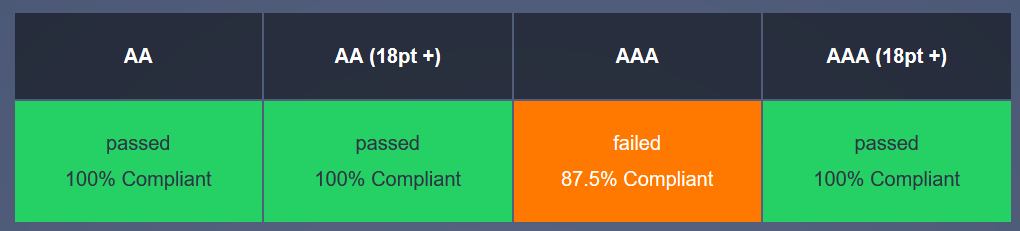
\includegraphics[width=0.475\textwidth]{bjornar/bg-image-h1.png}}
        \subfigure[Liten tekst]{\label{fig:analysis-current-a11y_bg-p}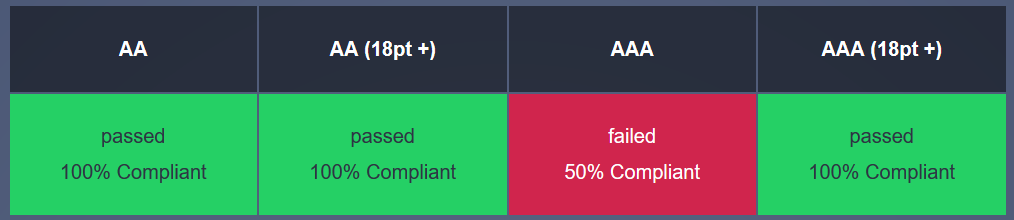
\includegraphics[width=0.475\textwidth]{bjornar/bg-image-p.png}}

        \caption{Testresultat}
        \label{fig:analysis-current-a11y_bg-h1_p}
    \end{center}
\end{figure}

Resultatet som vi ser i figur \ref{fig:analysis-current-a11y_bg-h1_p} viser at teksten i headeren har bra nok kontrastforhold for å passere kravet for AA, men ikke AAA. 

\subsection{Qualys SSL Server Test}
SSL Server Test\footnote{\url{https://www.ssllabs.com/ssltest/}} er en tjeneste som tester SSL og TLS sertifikater. Resultatet på testen ble en A. Dette er bra, men nettstedet burde få et bedre resultatet som A+ eller A++. Det kreves hverken mye tid eller ressurser for å oppnå dette.

\begin{figure}[H]
    \centering
    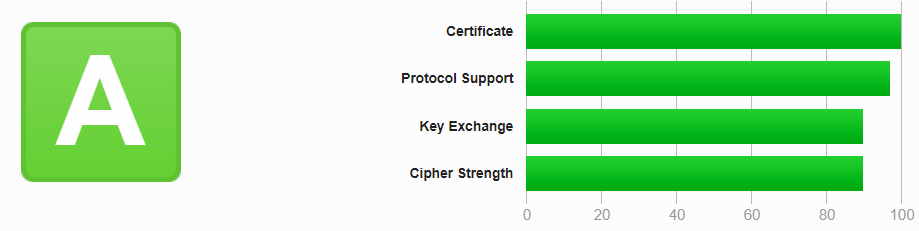
\includegraphics[width=\textwidth]{bjornar/ssllabs.png}
    \caption{Sertifikat score}
    \label{fig:analysis-current-ssl}
\end{figure}

\subsection{Test med skjermleser}
Brukervennligheten via skjermleser ble også testet. Nettsiden ble testet med skjermleseren NVDA\footnote{\url{https://www.nvaccess.org/about-nvda/}}. Det var enkelt å navigere seg rundt på nettsiden. Innholdet kom i en logisk rekkefølge og det var lett å navigere seg mellom elementene. Det eneste problemet var kontaktskjema, som er ganske viktig ettersom målet med nettsiden er at potensielle kunder skal ta kontakt. En annen faktor som manglet var en \q{skip to main content}-link.

\subsection{Google Transparency Report - Safe Browsing: malware and phishing}
Til slutt sjekket vi om nettsiden har skadevare på seg med en tjeneste fra Google\footnote{\url{https://transparencyreport.google.com/safe-browsing/search?url=https://sirkusmedia.no&hl=en-US}}. Her ble det ikke gjort noen funn, noe som selvfølgelig er positivt.

\subsection{Konklusjon}
Ut i fra testene gjort med Google Chrome DevTools, Google Lighthouse og Checkbot kan vi konkludere med at nettsiden er rask. På testen gjort ved høgskolen laster siden inn på under 1 sekund i gjennomsnittet, noe som er meget bra. Siden får over 70\% i poengsum fra Google Lighthouse og Checkbot. Med relativt enkle forbedringer, kan vi få denne summen opp til mellom 90-100\%.

Når det kommer til universell utforming gjør Sirkus Media det bra og følger de lover og regler som gjelder i Norge vedrørende dette. Vi ser likevel at kontrastforholdene på siden er gode nok for kravene til nivå AA, men ikke helt for AAA. Dette er noe som kan forbedres.

Totalt sett gjør nettstedet til Sirkus Media det bra på testene som vi kjørte den gjennom. Som tidligere nevnt er hovedgrunnen til dette at dagens nettsted består av kun en forside og lite informasjon. Dette begrenser muligheten for feil. Det vil være en utfordring å gjøre det like bra i disse testene med et nettsted som består av flere sider, mer innhold og kompleks funksjonalitet.

\section{Konkurrentanalyse}

Målet med konkurrentanalysen er å finne inspirasjon til nettstedet vi skal utvikle ved å se på allerede eksisterende løsninger. Hvem er oppdragsgiver sine konkurrenter? Hvordan type løsning har disse valgt? Hvilke styrker og svakheter har løsningene? Analysen er først og fremst gjort av gruppen med vekt på å se det fra en vanlig bruker sitt perspektiv, men noen tekniske faktorer har også blitt vurdert.

\subsection{Teknisk analyse}
For å vurdere de tekniske faktorene har vi brukt Google Lighthouse til å sjekke hvor raskt nettstedene lastes inn, beste praksis og SEO. I tillegg ble WAVE \footnote{Web Accessibility Evulation Tool. http://wave.webaim.org/} brukt til å sjekke om nettstedene følger kravene for loven om universell utforming og tilgjengelighet.

\subsection{Konkurrentene}
Sirkus Media har mange konkurrenter, deriblant alle firmaer som driver mediebyråvirksomhet. Etter samtale med Hans Christian Hymer \footnote{Samtale med oppdragsgiver (16.01.2019)} fikk vi oppgitt 3 bedrifter som blir ansett som Sirkus Media sine største konkurrenter. Det er følgelig disse konkurrentene vi har valgt å analysere.

\subsection{TACTIC™ Real-Time Marketing}
Nettstedet til TACTIC™ Real-Time Marketing ligger på følgende domene; https://tacticrealtime.com. Se figur \ref{fig:competitors-tacticrealtime.com} for bilde av nettstedet.

\subsubsection{Førsteinntrykk}
Førsteinntrykket er at nettstedet fremstår ryddig og profesjonelt. Det første som møter deg er et stort bakgrunnsbilde. Bilde dekker hele skjermen og har en tittel og en underoverskrift. Headeren består også av en knapp der du kan trykke på \q{Request a demo}. Helt øverst på forsiden er logoen til Tactic og en meny. Til høyre er det en knapp som gir deg muligheten til å se på en video. 

\begin{figure}[H]
    \centering
    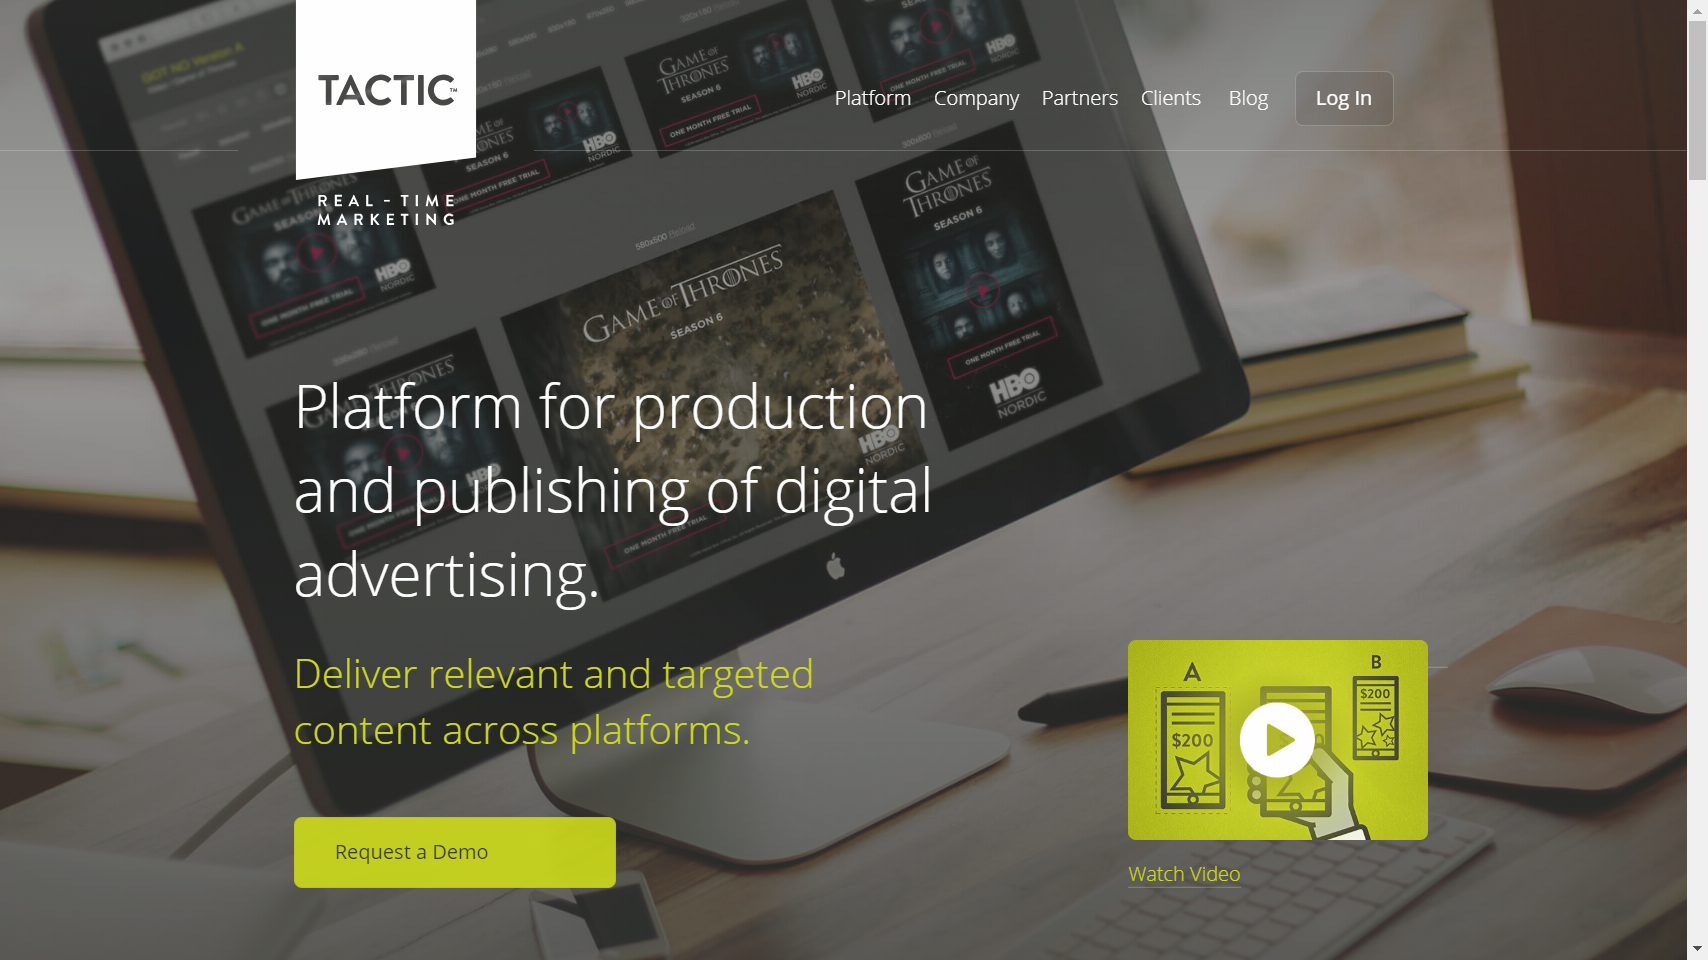
\includegraphics[width=\textwidth]{line/tacticrealtime_com_(1366x768).png}
    \caption{tacticrealtime.com}
    \label{fig:competitors-tacticrealtime.com}
\end{figure}

\subsubsection{Forside og undersider}

Forsiden består av bakgrunnsbilde som inneholder logo, meny, overskrifter og en video.  
Deretter kommer det en beskrivende tekst om firmaet, informasjon om plattformen, logo av ledende  Ad-servers og DSP's, partnerprogram og utvalgte kunder. Siden avsluttes med en \q{Contact us}-seksjon.

Nettstedet består også av følgende undersider:
\begin{itemize}
\item Platform
\item Company
\item Partners
\item Clients
\item Blog
\end{itemize}

\subsubsection{Teknisk analyse}

\begin{figure}[H]
    \begin{center}
        \subfigure[Google lighthouse]{
            \label{fig:competitors-lighthouse-summary-tacticrealtime.com}
            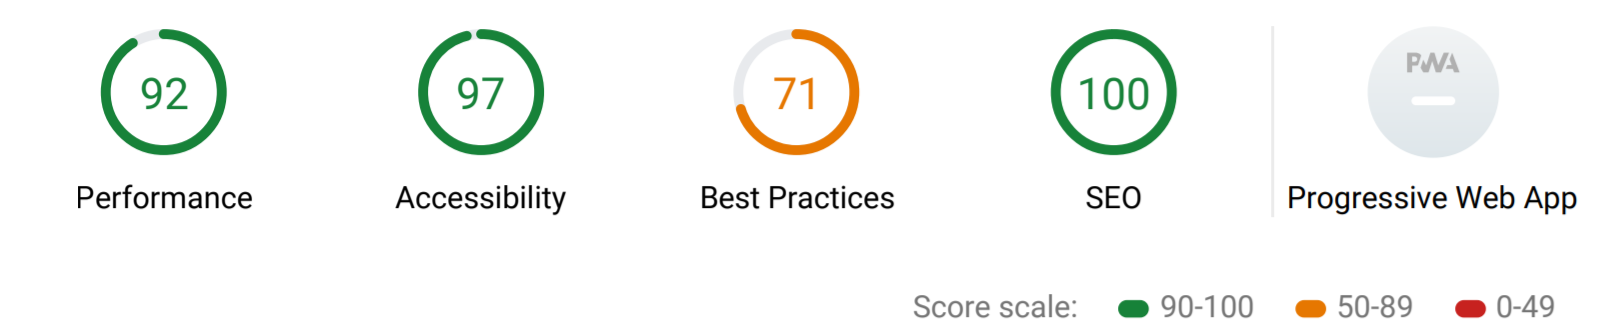
\includegraphics[width=0.7\textwidth]{line/tacticrealtime_com-lighthouse.png}
        }
        \rulesepv
        \subfigure[WAVE]{
            \label{fig:competitors-wave-summary-tacticrealtime.com}
            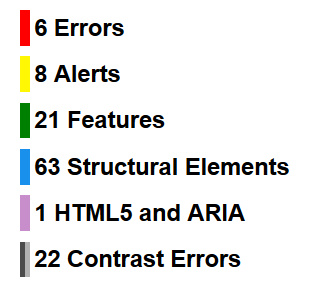
\includegraphics[width=0.2\textwidth]{line/tacticrealtime_com-wave.png}
        }
        
        \label{fig:competitors-tech_analysis-tacticrealtime.com}
        \caption{Resultat fra teknisk analyse av tacticrealtime.com}
    \end{center}
\end{figure}

Etter å ha gjennomført testen til Google Lighthouse, viste det seg at TACTIC var den desidert beste på alle punkter av de 3 konkurrentene. Restultatene fra Google Lighthouse kan man se i figur \ref{fig:competitors-lighthouse-summary-tacticrealtime.com}. Bedriften gjør relativt få feil med tanke på ytelse. Feilene som gjelder \q{Eliminate render-blocking resources}\footnote{Hva vil dette si?} og \q{Serve static assets with an efficient cache policy}\footnote{Hva vil dette si?} burde rettes opp. Vi kan se at siden lastet inn på 2,7 sekunder. Fikser man de overnevnte feilene, vil man kunne mer enn halvere innlastningstiden i følge rapporten.

Når det kommer til \q{Best Pracices}, så er det et par forbedringer TACTIC burde gjort. De burde benytte HTTP2, i stedet for HTTP \footnote{HTTP2 er bakoverkompatibel, så ingen grunn til å ikke bruke det. Samt at det pleier å være 1 linje med kode for å skru på for de fleste web-servere.}. Det linkes også til et JavaScript-bibliotek med kjente sikkerhetshull. Dette burde man på ingen måte gjøre.

På SEO-delen av testen fikk TACTIC 100 av 100 poeng og det er derfor ingenting å påpeke her.

Full rapport for Google Lighthouse kan leses i vedlegg X1.

Figur \ref{fig:competitors-wave-summary-tacticrealtime.com} viser resultatene fra WAVE. Fra resultatene ser man at Tactic fikk 6 feilmeldinger når det kommer til universell utforming. I tillegg har nettsiden deres 22 kontrastfeil. 

\subsubsection{Styrker}
En stor fordel er at nettstedet gir et bra førsteinntrykket. Dette fordi nettstedet fremstår som profesjonelt. Førsteinntrykket er dermed med på å styrke brukerens inntrykk av bedriften. Nettstedet har også god oppbygning og struktur. Løsningen har også en sterk profil, hvor det er ganske tydelig at det er grønn som er primærfargen til selskapet.

\subsubsection{Svakheter}
Noe som kan være en svakhet er at hele nettstedet er på engelsk og i tillegg er på et .com-domene. Disse to faktorene kan forvirre brukerne. En av grunnen til dette er at det er vanskelig å skjønne at dette er et firma som er lokalisert i Oslo. En annen svakhet er at det er lite luft rundt noen elementer, som fører til at nettstedet fremstår som kompakt og mer rotete. Det er heller ikke samme mengde luft over og under elementene. Dette er også med på å trekke ned helhetsinntrykket. Det er heller ikke så lett å bevege seg rundt på nettstedet ved hjelp av tastaturet ettersom TACTIC har fjernet all visuell indikasjon for fokus. Dette gjør at nettsiden ikke oppfyller noe som er et krav i loven om universell utforming og tilgjengelighet. I tillegg får nettstedet mange kontrastfeil, som også bryter lovkravet om universell utforming.

\subsection{Marketer Technologies AS}
Nettstedet til Marketer Technologies AS ligger på følgende domene;
https://marketer.tech/. Se figur \ref{fig:competitors-marketer.tech} for bilde av nettstedet.

\subsubsection{Førsteinntrykk}
Førsteinntrykket av nettstedet er positivt, fordi den fremstår som ryddig og profesjonell. Det første som møter deg er headeren\footnote{Hodet til nettstedet} til nettstedet, som inneholder logoen til firmaet og en meny. Under menyen er en tittel, en underoverskrift og to lenker. Headeren inneholder også et ikon for chat. Det at kunder enkelt kan ta kontakt med firmaet kan virke betryggende, og kan være med å øke troverdigheten til bedriften.

\begin{figure}[H]
    \centering
    
\includegraphics[width=\textwidth]{line/marketer_tech_(1366x768).png}
    \caption{marketer.tech}
    \label{fig:competitors-marketer.tech}
\end{figure}

\subsubsection{Forside og undersider}

Forsiden, i tillegg til headeren, består av logo til noen utvalgre kunder, prosessen til Marketer, animasjoner, resultater fra tidligere prosjekter og en presentasjon av deres løsninger. Helt nederst på siden kommer bunnfeltet, der organisasjonsnummeret, kontaktinformasjon og adresse blir presentert.

Nettstedet består også av følgende undersider:
\begin{itemize}
\item Solutions
\item Company
\item Customers
\item Blog
\item Careers 
\item Contact
\item Book demo
\end{itemize}

\subsubsection{Teknisk analyse}
\begin{figure}[H]
    \begin{center}
        \subfigure[Google lighthouse]{
            \label{fig:competitors-lighthouse-summary-marketer.tech}
            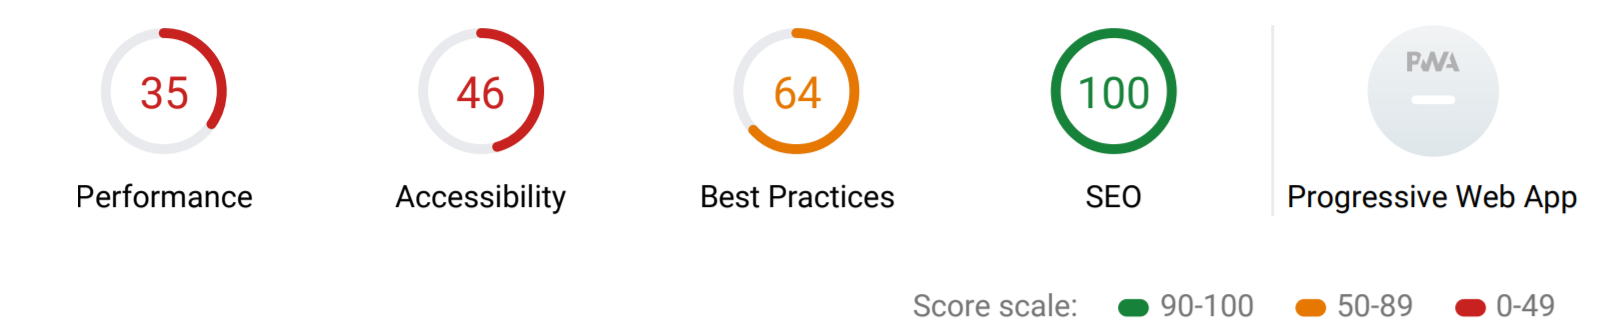
\includegraphics[width=0.7\textwidth]{line/marketer_tech-lighthouse.png}
        }
        \rulesepv
        \subfigure[WAVE]{
            \label{fig:competitors-wave-summary-marketer.tech}
            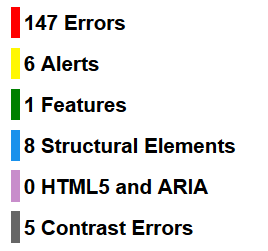
\includegraphics[width=0.2\textwidth]{line/marketer_tech-wave.png}
        }
        
        \label{fig:competitors-tech_analysis-marketer.tech}
        \caption{Resultat for teknisk analyse av marketer.tech}
    \end{center}
\end{figure}

Figur \ref{fig:competitors-lighthouse-summary-marketer.tech} viser resultatene fra testen gjort med Google Lighthouse. Her kom Marketer dårligst ut. Testen påpeker flere feil på punkter vedrørende ytelse, tilgjengelighet og beste praksiser. Det tar Google 5,3 sekunder å laste inn nettstedet, noe som er relativt tregt, men det er raskere enn Inviso.no. Selv om Marketer sin side laster inn raskere, så får den en dårligere poengsum på ytelse. Dette fordi det tar hele 15,2 sekunder før siden blir beregnet som interaktiv \footnote{\q{Time to Interactive} i Google Lightouse rapporten}. Marketer burde ta samme grep som TACTIC, i tillegg til å fjerne ubrukt CSS, servere skalerte bilder og vurdere å redusere antall animasjoner.
Full rapport for Google Lighthouse kan leses i vedlegg X2.

Figur \ref{fig:competitors-wave-summary-marketer.tech} viser WAVE-resultatene. Her kommer det frem at løsningen har 5 kontrastfeil og hele 147 feil når det kommer til universell utforming og tilgjengelighet. 135 av disse feilmeldingene er manglende bruk av alt-tekster.

\subsubsection{Styrker}
En av styrkene er at nettstedet gir et bra førsteinntrykk. Det er også et nettsted som skiller seg ut og er gjennomført. En annen styrke er at løsningen inneholder chat, der kunder enkelt kan ta kontakt. Profilen er også klar og tydelig, og det er åpenbart at bedriften har sort som primærfarge og turkis som aksentfarge.

\subsubsection{Svakheter}
En ulempe er at nettstedet består av flere store filer, som fører til at nettstedet oppleves som tregt. En annen svakhet er at løsningen får mange feil når det kjøres tester på universell utforming og tilgjengelighet. Det er i tillegg vanskelig å navigere seg rundt på nettstedet ved hjelp av kun tastatur.


\subsection{Inviso AS}
Nettstedet til Inviso AS ligger på følgende domene;
https://www.inviso.no/. Se figur \ref{fig:competitors-inviso.no} for bilde av nettstedet.

\subsubsection{Førsteinntrykk}
Førsteinntrykket av nettstedet er at den fremstår som rotete. Hovedgrunnen til dette er at det er mange elementer og mye som skjer i headeren. Logoen og noe av teksten på bakgrunnsbilde er også vanskelig å se på grunn av det dårlige kontrastforholdet. 

\begin{figure}[H]
    \centering
    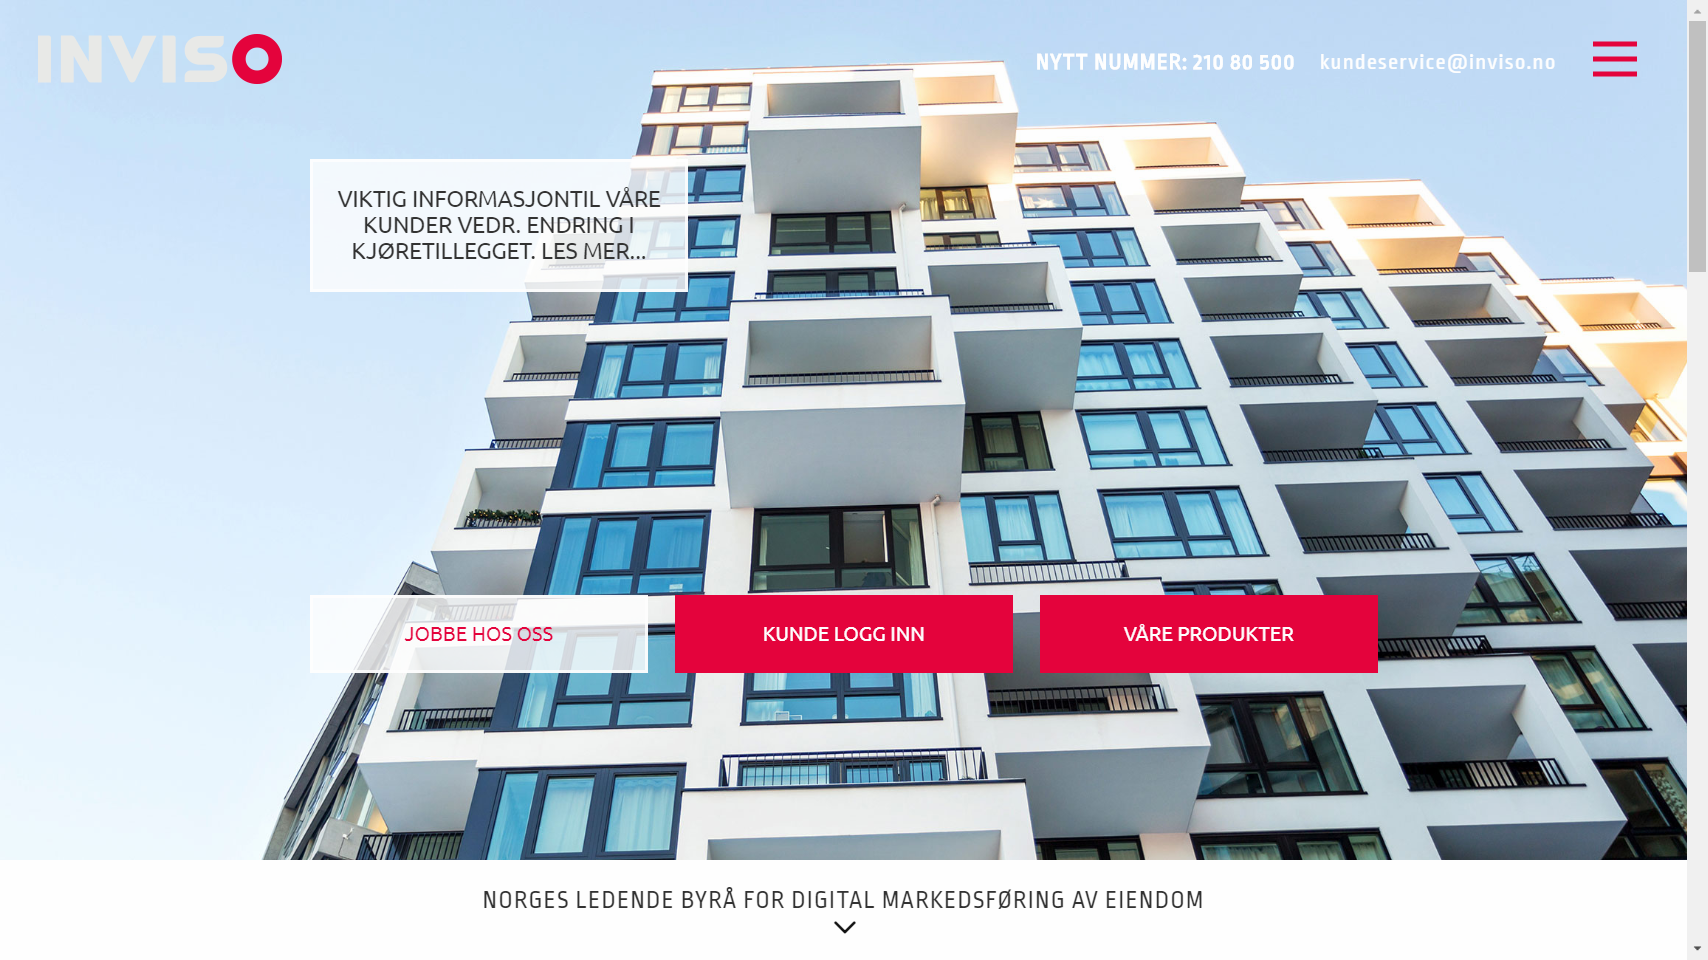
\includegraphics[width=\textwidth]{line/inviso_no_(1366x768).png}
    \caption{inviso.no}
    \label{fig:competitors-inviso.no}
\end{figure}

\subsubsection{Forside og undersider}
I tillegg til headeren består forsiden av \q{Om oss}-tekst, deres tjenester og utvalgte kunder. 

Nettstedet består også av følgende undersider:
\begin{itemize}
\item Inviso
\item Våre produkter
\item Kontakt
\item Galleri
\item Verktøy
\item Nyheter
\end{itemize}


\subsubsection{Teknisk analyse}

\begin{figure}[H]
    \begin{center}
        \subfigure[Google lighthouse]{
            \label{fig:competitors-lighthouse-summary-inviso.no}
            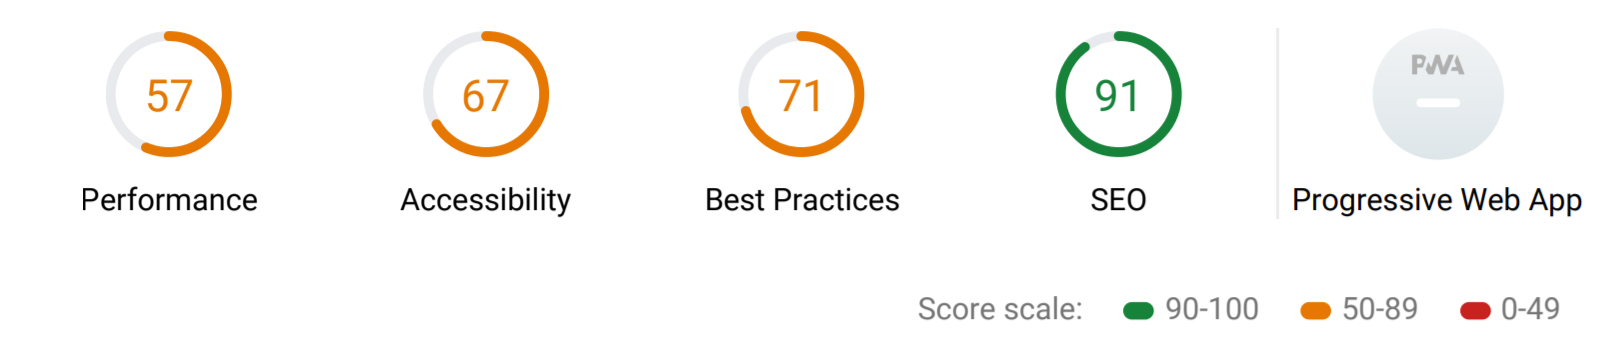
\includegraphics[width=0.7\textwidth]{line/inviso_no-lighthouse.png}
        }
        \rulesepv
        \subfigure[WAVE]{
            \label{fig:competitors-wave-summary-inviso.no}
            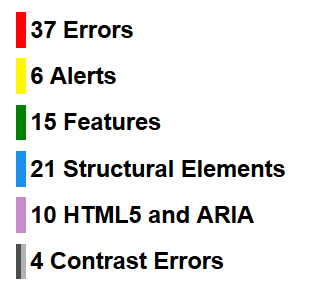
\includegraphics[width=0.2\textwidth]{line/inviso_no-wave.png}
        }
        
        \label{fig:competitors-tech_analysis-inviso.no}
        \caption{Resultat for teknisk analyse av inviso.no}
    \end{center}
\end{figure}

Figur \ref{fig:competitors-lighthouse-summary-inviso.no} viser resultatene fra testen gjort av Google Lighthouse. Her havnet Inviso midt på treet og kom dermed på andreplass av de tre konkurrentene. Bedriften får en helt grei poengsum i gjennomsnitt. Når det kommer til ytelse, bør de ta samme grep som både TACTIC og Marketer. Hovedproblemet her er at bildene serveres i en lite egnet filtype, og kan enkelt løse ved å velge en filtype som er mer egnet. Ved å fikse dette kan de hente inn hele 4,2 sekunder av den totale innlastningstiden på 6,7 sekunder.

På test delen vedrørende tilgjengelighet kommer det frem av Inviso burde forbedre kontrastforhold på deler av siden sin.

Ingenting spesielt å påpeke ved SEO, men Inviso burde absolutt ta en titt på hvilke JavaScript-biblioteker de bruker, ettersom Google kan melde om hele 5 kjente sikkerhetshull er tilgjengelig på siden. Full rapport for Google Lighthouse kan leses i vedlegg X3.

Ved å kjøre test via WAVE oppgir resultatet at nettstedet har 4 kontrastfeil. Nettstedet får også 37 feilmeldinger når det gjelder universell utforming. Figur \ref{fig:competitors-wave-summary-inviso.no} viser resultatene fra WAVE-testen.

\subsubsection{Styrker} 
En av styrkene er at nettstedet har en bra profil. Det er lett å skjønne at rød er primærfargen til Inviso. En annen positiv side er at det tekstlige innholdet på siden er godt skrevet og får bedriften til å fremstå profesjonelt.

\subsubsection{Svakheter}
En svakhet er at det er for mye informasjon i headeren. Dette kan bidra til at førsteinntrykket blir dratt ned. En annen stor svakhet er at nettstedet får mange feil når man kjører tester når det gjelder universell utforming og tilgjengelighet. Det faktum at nettsiden har en mobil-meny på fullversjon av siden, trekker også ned fordi dette gjør brukeropplevelsen dårligere.

\subsection{Konklusjon}
Felles for alle 3 konkurrentene er at ingen av de følger loven om universell utforming og tilgjengelighet. Universell utforming er lovpålagt i Norge \footnote{\url{https://lovdata.no/dokument/SF/forskrift/2013-06-21-732}}, og vår løsning kommer derfor til å følge disse kravene. 

En annen faktor konkurrentene har til felles er at de presenterer sine kunder og/eller partnere. Dette bør også Sirkus Media gjøre. Presentasjon av kundeforhold med kjente firmaer er tillitsvekkende og kan skape bedre troverdighet blant brukerne. \footnote{Kilde?}

Figur \ref{fig:competitors-mobile} viser at alle konkurrentene har gått for samme løsning når det kommer til design på mobil. Alle har bedriftens logo oppe til venstre og et meny ikon til høyre. Undersøkelser \footnote{Kilde: Luke Wroblewski, en internasjonalt anerkjent brukeropplevelsesdesigner \url{https://www.lukew.com/ff/entry.asp?1945}} viser at dette er langt fra den mest optimale løsningen. Planen er derfor at vår løsning skal ha en annen struktur.

Konkurrentene har gode løsninger, men også en del svakheter som har blitt påpekt i denne analysen. Konkurrentanalysen har vært nyttig fordi den både har ført til at gruppen har fått inspirasjon til deler av den løsningen som skal utvikles og samtidig gitt en pekepinn på hva som bør gjøres annerledes.

Studentgruppen har satt som mål å få minst like bra score på testen til Google Lighthouse, som gjennomsnittsscoren til de utvalgte konkurrentene.

\begin{figure}[bh]
    \begin{center}
        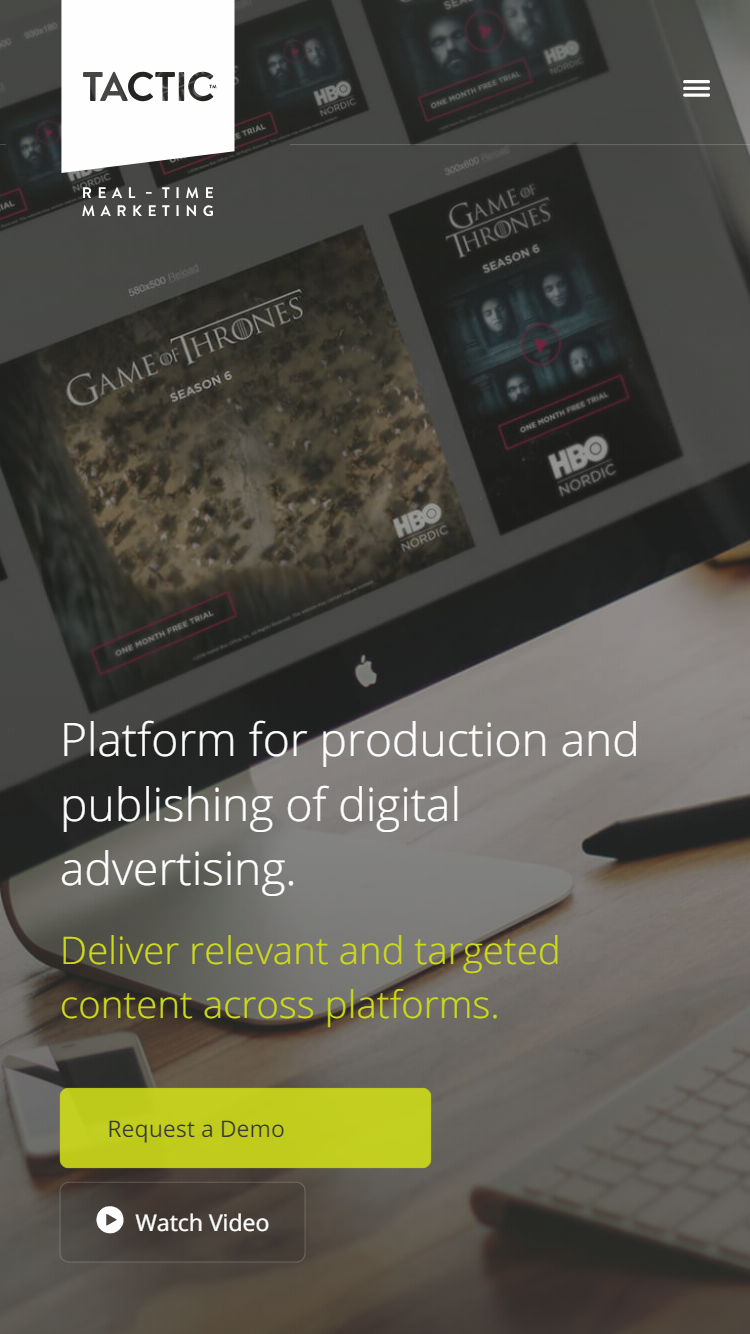
\includegraphics[width=0.3\textwidth]{line/tacticrealtime_com_(iPhone_6_7_8).png}
        
\includegraphics[width=0.3\textwidth]{line/marketer_tech_(iPhone_6_7_8).png}
        
\includegraphics[width=0.3\textwidth]{line/inviso_no_(iPhone_6_7_8).png}
        \caption{Alle nettstedene er mobiltilpasset}
        \label{fig:competitors-mobile}
    \end{center}
\end{figure}




\section{Teknologier}
Når det kommer til utvikling av nettsteder finnes det mange ulike teknologier, systemer og verktøy som kan benyttes for å få det samme resultatet. Derfor er det viktig å kartlegge brukerens behov og deretter sette ønskede kvalifikasjoner og krav, slik at de valgte verktøyene er tilpasset dette. Basert på de foregående analysene i dette kapittelet har studentgruppen kommet frem til et sett med minimumskrav. Videre blir passende verktøy og tilhørende teknologier presentert.

\subsection{Krav til teknologier}
Følgende sett med minimumskrav er satt med basis i den foregående analysen:


\subsection{Designmønster}
\subsection{Verktøy til grafisk design}
\subsection{Verktøy til back-end}
\subsection{Verktøy til front-end}
\subsection{Andre verktøy}
\subsection{Tilhørende teknologier og begreper}
\subsection{Verktøyanalyse}

\subsubsection{Laravel}
Laravel\footnote{\url{https://laravel.com/}} er et PHP-rammeverk, med åpen kildekode, som brukes til å lage webapplikasjoner og andre nettsteder. Rammeverket baserer seg på Symfony\footnote{Avsnitt \ref{sec:tools-symfony}} og følger Model-view-controller\footnote{Avsnitt \ref{sec:tools-mvc}} (MVC) designmønsteret.
Laravel kommer med innebygde funksjoner for autentisering, modeller, visninger, sesjoner, ruting og andre funksjoner som en \textit{templating engine} kalt Blade\footnote{\url{https://laravel.com/docs/5.7/blade}}.

%%% VI SER PÅ FORDELER OG ULEMPER SENERE %%%
%\textbf{Fordeler}
%\begin{itemize}
%    \item Laravel er veldig raskt i forhold til CMS (Content Management Systems).
%    \item Har funksjoner som autentisering og autorisasjon.
%    \item Alt kan tilpasses og styres hvordan tingene fungerer.
%    \item Databasen kan brukes eller utformes på egen måte.
%\end{itemize}

%\textbf{Ulemper}
%\begin{itemize}
%    \item I Laravel må SEO definere egne ruter, og det tar mye arbeid å utvikle et nettsted som hovedsakelig er avhengig av innhold.
%    \item Laravel rammeverk er litt komplisert og krever mer kunnskap.
%    \item Laravel er mindre fleksibel for å oppdatere innholdet.
%\end{itemize}

%Fordeler og Ulemper av laravel ble tatt i forhold til CMS.
%Kilde: \url{https://www.educba.com/laravel-vs-wordpress/}

\subsubsection{Symfony}
\label{sec:tools-symfony}
Symfony er et webapplikasjonsrammeverk og er et sett med gjenbrukbare komponenter og biblioteker skrevet i PHP. \cite{symfony19wis}

\subsubsection{MVC}
\label{sec:tools-mvc}
Model-View-Controller (MVC)\footnote{\url{http://www.dgp.toronto.edu/~dwigdor/teaching/csc2524/2012_F/papers/mvc.pdf}} er et designmønster som deler et program inn i tre hovedkomponenter: modell, visning og kontroll.\cite{burbeck87aps} Oppbygningen kan enkelt forklares ved hjelp av et eksempel fra Matteo publisert på dev.to:
Matteo J. (2018, Mars 16) Re: Explain MVC like I'm five [Blogg kommentar]\footnote{\url{https://dev.to/matteojoliveau/comment/2ikd}}
\begin{quote}
    You walk in a McDonald and you order at the big interactive touchscreen.
    The screen is the View, and you ask for your meal there.
    The order is passed to the operator, who is the Controller, that will go in the kitchen and fetch a burger (your wanted resource) of the type (Model) you asked, then deliver it back to you.
\end{quote}
%Typisk flyt er at det kommer inn en forespørsel som går til kontrolleren. Den tolker forespørselen og behandler den ved å hente og endre data via modell. Til slutt sendes det et svar til visning.

\textbf{Modell} (Model) representerer de forskjellige type ressurser en applikasjon har. Her beskrives hver ressurs, hvordan den er oppbygd og hva som kan gjøres med den.

\textbf{Visning} (View) håndterer brukerinteraksjon og presentasjon av data. Er ofte et grafisk brukergrensesnitt.

\textbf{Kontrolleren} (Control) delen er ansvarlig for å koordinere forespørsler og svar.

\subsubsection{GNU/Linux}
GNU/Linux er en familie med Unix-lignende operativsystemer som baserer seg på Linux-kjernen og en del programvare fra GNU-prosjektet.
I denne familien finner vi blant annet Ubuntu, Debian, Fedora, Red Hat Linux og Arch Linux.
Kilder: \url{https://www.kernel.org} \url{https://www.gnu.org/} \url{https://www.ubuntu.com/} \url{https://www.debian.org/} \url{https://getfedora.org/} \url{https://www.redhat.com/en/topics/linux} \url{https://www.archlinux.org/}

\subsubsection{Nginx}
Nginx er en gratis HTTP-server med åpen kildekode. Nginx har mulighet til å håndtere høy belastning av HTTP-forespørsler. Programmet er tilgjengelig på operativsystemer som Windows, Mac OS og Solaris. I tillegg er Nginx tilgjengelig på operativsystemer som er basert på GNU/Linux eller BSD.

Kilde: Nedelcu, C. (2010). Nginx HTTP Server: Adopt Nginx for Your Web Applications to Make the Most of Your Infrastructure and Serve Pages Faster Than Ever. Packt Publishing Ltd.

\subsubsection{PHP}
PHP (rekursiv akronym for PHP Hypertext Pre-processor) er et skriptspråk som er spesielt egnet for webutvikling og kan legges inn i filer sammen med HTML. PHP er et serverside programmeringsspråk og kan brukes til å lage dynamiske og interaktive nettsteder. PHP er gratis og plattformuavhengig, samtidig som det er  er raskt og fleksibelt. Det kan installeres i pakker med webserver og database. Eksempelvis LAMP, LEMP, WAMP og XAMPP. PHP er også mulig å installere enkeltstående. 

Kilde: \url{http://php.net/}

\subsubsection{Sesjoner}
En sesjon\footnote{\url{https://ieeexplore.ieee.org/abstract/document/8392612}} (session) er en samling av data lagret på en webserver. En webserver tildeler en ID til hver bruker som sender forespørsler via en nettleser. ID-en lagres som en informasjonskapsel i nettlesern til brukeren. Alle nye forespørsel vil så identifiseres av ID-en som er lagret hos brukeren.

\subsubsection{phpMyAdmin}
phpMyAdmin\footnote{\url{https://www.phpmyadmin.net/}} er et gratis og webbasert administrasjonsverktøy for MySQL og MariaDB databaser. Verktøyet er skrevet i PHP og JavaScript. Med phpMyAdmin kan man lage, endre og slette databaser, tabeller og felter. Annen funksjonalitet kan være å utføre SQL-setninger, administrere nøkler og privilegier og eksportere data til ulike formater.

\subsubsection{MariaDB}
MariaDB er et relasjonsdatabasesystem basert på MySQL, som er gratis og har åpen kildekode. Systemet funker som en \textit{drop-in} erstatning for MySQL.

Kilde \url{https://mariadb.org/}

\subsubsection{CSRF}
Cross site request forgery\footnote{\url{https://ieeexplore.ieee.org/abstract/document/5283085}} (CSRF) er angrep som tvinger brukere til å utføre uønskede handlinger på en nettside der brukeren er logget inn, via en annen nettside. For eksempel: hvis brukeren er logget inn på Facebook.com, og går til Twitter.com. Da kan Twitter laste inn et bilde som dette: \lstinline{<img src="https://facebook.com/delete-my-account">}. Dette vil da sende en forespørsel til den linken, som kan føre til sletting av konto. Om Facebook ikke har implementert mottiltak for slike angrep, vil denne forespørselen tolkes som om den kommer direkte fra brukeren.

\subsubsection{CI \& CD}
CI står for continuous integration og CD står for continuous delivery. CI/CD\footnote{\url{https://www.atlassian.com/continuous-delivery/principles/continuous-integration-vs-delivery-vs-deployment}} er en metode som lar utviklere implementere og levere kodeendringer raskt og pålitelig.

\subsubsection{Buddy}
Buddy\footnote{\url{https://buddy.works}} er en webbasert applikasjon for CI og CD. Applikasjonen lar utviklere bygge, teste og distribuere nettsider og programkode automatisk når kildekoden oppdateres. For eksempel er det mulig å koble Buddy til et nettsteds kildekode via Git. Når koden til nettstedet oppdateres, vil Buddy automatisk detektere endringer og starte en byggeprosess. Når byggeprosessen er ferdig kjøres det automatisk tester på koden, som verifiserer at alt fungerer. Deretter vil Buddy laste koden opp til en server og oppdatere nettstedet som ligger ute på nett. Dette skjer gjerne gjennom Docker\footnote{\url{https://www.docker.com/}} sammen med Kubernetes\footnote{\url{https://kubernetes.io/}}.

\subsubsection{Axios}
Axios\footnote{\url{https://github.com/axios/axios}} et et JavaScript-bibliotek for en promise-basert\footnote{\url{https://leanpub.com/exploring-es6/}} HTTP-klient som kan kjøres i nettlesere og Node.Js. Biblioteket gjør det enklere å lage og behandle asynkrone forespørsler.

\subsubsection{Git}
Git er et system for versjonskontroll. Et versjonskontrollsystem blir hovedsaklig brukt under utvikling av software og nettsteder. Det kan også brukes til andre type prosjekter som grafisk design og skriving av dokumenter.

Ved å bruke Git opprettes det historikk over alle endringer, samt en sikkerhetskopi av alle versjoner av filene.

En annen fordel ved å bruke Git er at det blir enklere å samarbeide med andre, uten å måtte tenke på at alle må sitte på nyeste versjon av filene.

KILDE (GIT OG GITHUB): \url{https://journals.plos.org/ploscompbiol/article?id=10.1371/journal.pcbi.1004668}
\url{https://searchitoperations.techtarget.com/definition/GitHub}

\subsubsection{Github}
GitHub.com er et nettsted for å hoste git repositories, og blir mye brukt for \q{Open Source}-prosjekter. 

Github er et sentralisert punkt for å samle en brukers repositories. Ved siden av å hoste repositories, lar GitHub brukere dele repositories med hverandre, lage informasjonssider om prosjektet og opprette saker (issues).
 
\subsubsection{Overleaf}
Overleaf\footnote{\url{http://web.simmons.edu/~wilsonjd/LIS488/website/OverleafTutorial.pdf}} er en tjeneste som brukes til å lage, redigere og dele akademiske artikler på nettet ved hjelp av LaTeX. Dette er et nettbasert tekstforfattings-program. 
Overleaf v2\footnote{\url{https://no.overleaf.com/learn/how-to/Working_Offline_in_Overleaf}} tilbyr synkronisering med GitHub og Dropbox.

\subsubsection{Ottomatik.io}
Ottomatik\footnote{\url{https://ottomatik.io/}} er en webbasert tjeneste for automatisk sikkerhetskopiering av filer og MySQL databaser.

\subsubsection{Amazon S3}
Amazon Simple Storage Service\footnote{\url{https://aws.amazon.com/s3/}} er en webbasert tjeneste som tilbyr objekt-lagring. Tjenesten tilbyr meget god skalerbarhet, datatilgjengelighet, sikkerhet og ytelse.

KILDE: https://dash.harvard.edu/handle/1/24829568

\subsubsection{HTTP/2}
HTTP/2\footnote{\url{https://www.rfc-editor.org/rfc/pdfrfc/rfc7540.txt.pdf}} er en revisjon av HTTP-nettverksprotokollen. HTTP er et sett med regler for overføring av filer (tekst, grafiske bilder, lyd, video og andre mediefiler). Et av de store målene med HTTP/2 var å tillate multipleksing.

\subsubsection{HTTPS}
HTTPS\footnote{\url{https://www.rfc-editor.org/rfc/pdfrfc/rfc2616.txt.pdf}} (Hypertext Transfer Protocol Secure) er en sikker versjon av HTTP-protokollen som overfører data på nett. HTTPS-protokollen krever at det opprettes en kryptert kanal mellom nettleseren og webserveren, slik at overføring mellom disse blir sikker.

\subsubsection{TLS}
Transport Layer Security er en kryptografisk protokoll. Dette er viktig for å sikre informasjon som overføres gjennom nettverk. TLS brukes i forskjellige tjenester som HTTPS, FTPS, VoIP og VPN.
Når en tjeneste bruker en sikker tilkobling, legges bokstaven S til tjenestens protokollnavn. For eksempel: HTTPS, SMTPS, FTPS, SHIPS.
SSL (Secure Socket Layer) er en utdatert forgjenger til TLS.

KILDE: Thomas, S. (2000). SSL and TLS essentials. New Yourk, 3.

\subsubsection{Let’s Encrypt}
Let’s Encrypt\footnote{\url{https://letsencrypt.org/}} er en gratis og åpen sertifikatautoritet som gir ut X.509-sertifikater for kryptering av transportlaget. Tjenesten leveres av ISRG (Internet Security Research Group).

\subsubsection{HTML}
Hypertext Markup Language\footnote{\url{https://www.w3.org/standards/webdesign/htmlcss}} er et markeringsspråk som brukes til å lage nettsidedokumenter. Det er et system som identifiserer og beskriver de forskjellige komponentene i et dokument som overskrifter, avsnitt og lister. HTML5 er den nyeste versjonen av HTML-standarden.

\subsubsection{CSS}
Casecading Style Sheet\footnote{https://www.w3.org/standards/webdesign/htmlcss} er et format for stilsett som beskriver utseendet i en applikasjon eller på et nettsted. CSS styrer blant annet fonter, farger, bakgrunnsbilder, linjeavstand og sidelayout. Formatet lar utviklere style innhold på en slik måte at brukere enklere kan identifisere hva det er, samt være i tråd med en bedrift eller person sin identitet.

\subsubsection{SASS}
Syntactically Awesome Style Sheets\footnote{\url{https://sass-lang.com/}} er en utvidelse av CSS. SASS gir mulighet til å bruke variabler, nestede regler, inline-import og mixins. Alt dette gjør det enklere å gjenbruke CSS syntaks. Med SASS er det mulig å lage stilark raskere. SASS er kompatibel med alle versjoner av CSS. Det er ingen nettlesere som kjører SASS, man må derfor kompilere SASS til CSS for å kunne bruke det på nettsider.

KILDE: Cederholm, D. (2013). Sass for web designers. A Book Apart.

\subsubsection{JavaScript}
JavaScript\url{https://developer.mozilla.org/en-US/docs/Web/JavaScript} er et programmeringsspråk som følger ECMAScript-spesifikasjonen. Det er mye brukt til å utvikle webapplikasjoner. Språket støttes av de fleste moderne nettlesere, og brukes til å manipulere elementene på nettsiden og stilene som er brukt på dem. JavaScript støtter objektorientert- og funksjonell programmering.

\subsubsection{React}
React\footnote{\url{https://reactjs.org/}} er et fleksibelt JavaScript-bibliotek for å bygge brukergrensesnitt, og brukes som visningslaget for webapplikasjoner som følger MVC. React har åpen kildekode og er utviklet av Facebook.

Alternativ kilde: \url{https://www.fullstackreact.com/assets/media/sGEMe/MNzue/30-days-of-react-ebook-fullstackio.pdf}

\subsubsection{REST-API}
Et API (programmeringsgrensesnitt) er et sett med funksjoner, prosedyrer, metoder eller klasser som brukes av dataprogrammer for å be om tjenester fra operativsystemet eller programvare som er på datamaskinen. En programmerer kan bruke API-er til å lage applikasjoner.

REST (Representational State Transfer) er en arkitektonisk stil for programvare. Et REST-API er et API som følger REST-stilen og de begrensninger som REST definerer.

KILDE: Masse, M. (2011). REST API Design Rulebook: Designing Consistent RESTful Web Service Interfaces. " O'Reilly Media, Inc.".
side 5 og 6

\subsubsection{NODE.JS ?????}

\subsubsection{Figma}
Figma\footnote{\url{https://www.figma.com/}} er et webbasert designverktøy som åpner muligheten for å samarbeide i sanntid. Med Figma er det også mulig å designe mockups og prototyper av applikasjoner og nettsider.

ekstra kilde: \url{https://www.xfive.co/blog/figma-best-designer-developer-cooperation/}

\subsubsection{Google Analytics}
\label{sec:google-analytics}
Google Analytics\footnote{\url{https://analytics.google.com/analytics/web/}} er en gratis, webbasert tjeneste som gir statistikk og grunnleggende verktøy for analyse av bruksdata, søkemotoroptimalisering og markedsføring.

\subsubsection{Google Lighthouse}
Google Lighthouse\footnote{\url{https://developers.google.com/web/tools/lighthouse/}} er et gratis verktøy for å sjekke kvaliteten på nettsider. Det analyserer nettsidens tilgjengelighet, hastighet og SEO, samt om nettsiden følger de beste praksiser både generelt sett og for progressive webapplikasjoner. Lighthouse kan kjøres via Google Chrome DevTools, en nettleserutvidelse i Google Chrome eller via nettsiden \url{https://web.dev/}.

\subsubsection{WAVE}
Web Accessibility Evaluation Tool\footnote{\url{https://wave.webaim.org/about}} er et verktøy som tester universell utforming hos nettsider og hvorvidt de følger visse punkter i WCAG 2.1-standarden og Section 508. Verktøyet er tilgjenglig som en nettleserutvidelse og som en webbasert tjeneste hos \url{https://wave.webaim.org/}.

\section{Testing}

\subsection{Funksjonell testing}
Funker nettstedet slik som Sirkus Media vil?

\subsection{Ikke funksjonell testing}
Funker nettstedet bra, teknisk sett?

\subsection{Brukertesting}
Hva syns brukere om nettstedet?






\section{Akademiske og tekniske dokumenter}

Akademiske og tekniske dokumenter ser noe forskjellige ut avhengig av fagfeltet. Likevel, en litt grundigere analyse avslører en felles hovedstruktur, som egentlig er ganske intuitiv\dots og omtrent lik den vi lærte på barneskolen: {\em Hode, kropp og hale}. Hver av disse hoveddelene består som regel av omtrent de samme elementene. 



\subsection{Mayfield Handbook of Technical \& Scientific Writing}
\label{sec:mayfield}

I følge engelsk terminologi deler man gjerne et dokument opp i {\em Front matter, Body og End (Back) matter}, og det gjøres konsekvent i
Mayfield Handbook of Technical \& Scientific Writing \cite{perelman97mht}. Denne utmerkede kilden finnes også på 
elektronisk form\footnote{\url{http://www.mhhe.com/mayfieldpub/tsw/home.htm}}. 
I kapittelet 
{\em Elements of Technical Documents}\footnote{\url{http://www.mhhe.com/mayfieldpub/tsw/elemtech.htm}}
blir den følgende generiske strukturen foreslått:

\begin{compactitem}
\item Front Matter
\begin{compactitem}
\item Title page
\item Abstract
\item Table of contents
\item List of figures
\item List of tables
\item List of terms
\item Acknowledgments
\end{compactitem}

\item Body
\begin{compactitem}
\item Introduction
\item Background
\item Theory
\item Design criteria
\item Materials and apparatus
\item Procedure
\item Workplan
\item Results
\item Discussion
\item Conclusion
\item Recommendations
\end{compactitem}

\item End Matter
\begin{compactitem}
\item References
\item Appendixes
\item Index
\end{compactitem}

\end{compactitem}

Hvert av punktene blir nærmere beskrevet, med mange eksempler på godt (og dårlig) innhold, og det anbefales på det sterkeste å  studere dette kapitellet nærmere. 

Denne strukturen er så nær man kommer en universell mal for en teknisk/vitenskapelig rapport.

\subsection{HiØ/IT}
\label{sec:hiof-it}

Ved HiØ/IT har man valgt å skille grovt sett mellom to typer dokumentasjon.
{\em Prosessdokumentasjonen} omfatter en forprosjektrapport samt individuelle refleksjonsnotater, og selve produktet er omtalt i
{\em hoveddokumentet}\footnote{\url{https://wiki.hiof.no/index.php/Bacheloroppgaven_-_Leveranser}}(eller rett og slett det vi kaller bacheloroppgaven).
Når det gjelder oppbygging og innhold er hoveddokumentet å regne som en typisk akademisk/teknisk rapport/artikkel:

\begin{compactitem}
\item Tittelside
\item Sammendrag
\item (Takk til)
\item Innholdsfortegnelse
\item (Liste over figurer)
\item (Liste over tabeller)
\item Introduksjon
\item Analyse
\item Design
\item Implementasjon
\item Evaluering
\item Diskusjon
\item Konklusjon
\item Referanser
\item Referanser
\end{compactitem}

\section{Skriveverktøy for store og komplekse dokumenter}

For å starte på et stort og komplekst dokument, vil mange åpne sin vanlige teksteditor og sette igang. Det går sjelden bra. Som ved alle typer større oppgaver, bør man velge sine verktøy med omhu.
Før man setter igang å lage et digitalt dokument, kan det være fornuftig å dvele litt ved hvordan dokumenter har blitt, og blir, produsert på tradisjonelt vis. 

\subsection{Forfatter, redaktør, typograf, trykkeri}

Tradisjonelt hersker det en streng arbeidsdeling innen produksjon av dokumenter, som f.eks. en bok, eller en avis. Forfatteren (eller journalisten) skriver såkalt {\rm brødtekst}, som rett og slett er tekst, skrevet for hånd, på skrivemaskin, eller talt inn på diktafon. I teksten er det gjerne markert ulike strukturelle elementer. Det er markert hvor et nytt avsnitt begynner, kanskje det står skrevet at her kommer det en illustrasjon, etc. Dette råmaterialet går gjerne til en redaktør, som kvalitetssikrer innholdet og tildels struktur, og eventuelt foreslår/foretar endringer. Deretter tar typografen (eller den grafiske formgiveren) over, og bestemmer skriftstørrelser, fonter, marger, linjeavstand etc. Til slutt går trykkoriginalen til trykkeriet\footnote{Her kan jo være på sine plass å tenke litt på XHTML og CSS, og hvor de har sine røtter\dots og da tenker jeg ikke på Håkon Wium Lie \smiley.}.

Denne framgangsmåten ivaretar en klar tredeling av arbeidet; innhold, struktur, og form. Innholdet, og grovstrukturen, bestemmes av forfatteren. Redaktøren sørger for å kvalitetssikre innholdet, og eventuelle justere strukturen. Den endelig formgivingen av dokumentet blir typografens rolle. Det er viktig å merke seg at alle disse tre rollene krever høy kompetanse innen helt forskjellige fagfelt. De fleste mener også at det er ganske unaturlig for en forfatter å legge ned mye tankearbeid i hvilken font og størrelse det bør være på overskriftene. På den annen side ville vel det ikke være rett at typografen blandet seg bort i innholdet.

\subsection{The curse of the cursor \\  \normalsize -eller- \\DTP: DeskTop Publishing eller Dom Tokigas Paradis? }

Og etterhvert kom datamaskinene, som tilsynelatende kunne gjøre ``alt'', og dermed begynte mange å gjøre ``alt'', selv. Teksteditorer og desktop publishing verktøy gjorde det mulig for at en person kunne stå for hele prosessen, både skrive, redigere, og formgi, uten å ha særlig kompetanse, ferdighet eller erfaring i noen av feltene.

Personlig husker jeg godt mitt første møte med DTP, tidlig i IT-utdannelsen. Oppgaven var å lage en liten avis, med bilder og det hele, ved hjelp av en søt liten Mac, som på et mysteriøst vis var knyttet sammen med en skriver som til og med skrev ut illustrasjoner og fotografier i grov oppløsning. Den blinkende markøren i teksteditoren var hypnotisk, halvt innbydende, halvt skremmende. Og så måtte man bare kaste seg ut i det. Skrive noen setninger, markere en del som ``bold'' og fontstørrelse 18, fin overskrift, et par ``enter'', forsette med vanlig font, nei, kanskje en litt mer fancy kalligrafifont, kanskje til og med blå? Og dermed var det gjort, forvirringen var total. Noe senere erfarte jeg at i enkelte svenske miljøer mente man at DTP sto for ``Dom Tokigas Paradis". Innen visse segmenter av reklamebransjen mener jeg fremdeles å se spor etter slike traumatiske møter med datastøttet publisering.

Man kan jo spørre seg om det egentlig er noen forskjell mellom et blankt ark, enten på et skrivebord eller i en skrivemaskin, og en blinkende markør øverst i venstre hjørne i en editor? Uansett svar, det blanke arket gir deg ikke anledning til å eksperimentere med fonter, marger, skriftstørrelse og plassering av bilder. Arket handler kun om innhold, og hvordan det skal struktureres, hvilken passasje som følger en annen, og hvor det begynner et nytt avsnitt.

\subsection{Programmering av dokumenter}

Et par år senere skal jeg produsere min første akademiske artikkel, i \LaTeX~med  AMS stilen. Hæh?

Det tok et par dager før jeg skjønte poenget. Skrive innholdet i filer (ark) i en editor uten formateringsmulighet, sette inn kryptiske kommandoer for å markere avsnitt eller matematiske uttrykk, sette sammen delene i en styrefil, legge til noen kommandoer som avgjorde hvordan dokumentet ble seendes ut. Deretter {\em kompilere} hele greia! Som så resulterte i  en DVI-fil\footnote{DVI: DeVice Independent}, som igjen kunne konverteres til alle mulige trykk- og printbare formater. Og det beste av alt, resultatet, rent formmessig, ble helt strøkent, akkurat som i lærebøkene og artikkelsamlingene.

Dette var jo akkurat som å programmere. Full kontroll.


\section{Digital dokumentproduksjon}

Vi foreslår et sett med minimumskrav til digitale dokumentverktøy, basert på  den forutgående analysen. Deretter gir vi kort beskrivelse av 
\LaTeX~ og OpenOffice Writer, som etter en kort vurdering er de to verktøyene som tilfredstiller de fleste av kravene.

\subsection{Generelle krav}
\label{sec:generelle-krav}

Kravene er utarbeidet delvis med basis i den forutgående analysen, men i hovedsak ut fra forfatterens erfaringer.

\vspace{1em}
\begin{compactdesc}
\item [Plattformuavhengighet] I et prosjekt med flere deltagere, er det direkte arrogant å forvente at alle skal bruke samme plattform, fordi valget av dokumentasjonsverktøy krever dette.
\item [Robusthet] En hovedrapport er ofte relativt stor, og tildels med komplekst innhold (figurer, tabeller etc). Det er ikke uvanlig at selv kostbare og vidt utbredte verktøy kræsjer i en slik kontekst, eller verre, begynner å oppføre seg inkonsistent og uforutsigbart Det å åpne et dokument, bare for å oppleve at formatering som ble foretatt kvelden før er ødelagt, er ingen særlig givende erfaring, særlig ikke hvis det er to timer til rapporten skal leveres inn.
\item [Maler/stiler] Det må kunne være mulig å skifte mal på et og samme dokument uten å gjøre ekstra tilpasninger. Dermed oppnår man et klart skille mellom innhold og utforming. Hvis f.eks. retningslinjene for hovedrapporten endrer seg, så er det bare å lage en ny mal og bruke denne.
\item [Oppsplitting]Det bør kunne være mulig å splitte dokumentet i mindre deler, f.eks. en fil for hvert kapittel. Delene må kunne knyttes sammen i et masterdokument. På denne måten vil det være lett å endre rekkefølgen på komponentene. Da er også strukturen uavhengig av det faktiske innholdet. Oppsplitting er også en forutsetning for å kunne jobbe distribuert, der de ulike deltagerne jobber parallelt på ulike deler av rapporten.
\item [Kryssreferanser]Det må være mulig å bruke dynamiske kryssreferanser, slik at man f.eks. kan referere til en nummerert figur. Hvis da nummeret til figuren endrer seg pga. av at det blir lagt inn en figur tidligere i dokumentet, så må referanse oppdateres automatisk.
\item [Bibliografi]De må være enkelt å referere til en ekstern samling bibliografiske referanser. Det også være enkelt å når som helst endre referansestil (f.eks. IEEE eller Harvard).
\item [Brukermasse]Det bør eksistere en stor og variert brukermasse, noe som i seg selv kan være en antydning om at verktøyet holder mål.
\item [Dokumentasjon]Verktøyet må være godt dokumentert, både den innebyggede dokumentasjonen, samt i ulike fora på nettet.
\item [Versjonskontroll]Det må være enkelt å håndtere versjonering, dvs. at man lett kan rekonstruere tidlige versjoner, og lett se hva som er endret fra versjon til versjon.
\item [Framtids/fortidssikker]Verktøyet bør kunne uten videre behandle dokumenter som er laget i tidligere versjoner. Dette vil også være en indikasjon på at dokumentet du jobber fremdeles ``lever'' i rimelig overskuelig framtid. 
\item [Stave/grammatikkontroll] Minimumskravet er at det er mulig å utføre effektiv stavekontroll, for ulike språk, ikke minst norsk bokmål. I tillegg vil det være et pluss om det er mulig å verifisere grammatikk.
\end{compactdesc}


\subsection{\LaTeX}

Klipt og limt fra Wikipedia\footnote{\url{http://no.wikipedia.org/wiki/LaTeX}}:

\begin{quotation}
\LaTeX~ er et typesettingssystem for dokumentproduksjon. Det skrives normalt LaTeX i dokumenter som ikke har hevet og senket tekst.
\LaTeX~ ble opprinnelig utviklet av Leslie Lamport i 1984 og tilbyr idag en lang rekke dokumentproduksjonspakker som f.eks. automatisk opprettelse av innholdsfortegnelser, lister med tabeller og figurer, inkludering av bilder, kryssreferanser, sideoppsett, bibliografier mm.


LaTeX~ baserer seg på at forfatteren av et dokument kun skal være forfatter av dokumentet og slippe å bry seg om utforming og hvordan ting ser ut; noe han normalt sett ikke er ekspert på uansett. Det forfatteren gjør er å dele opp dokumentet i logiske strukturer før han lar LaTeX~ ta seg av selve oppsettet. LaTeX~ ansees ofte som WYSIWYM (det du ser er det du mener) fremfor WYSIWYG (det du ser er det du får) editor. Dette fører til at det ofte anerkjennes som overlegent fremfor andre skriveprogrammer grunnet at endringer som påvirker hele dokumentet er meget enkle å gjennomføre. De trenger ofte bare en endring et sted, så er endringen gjennomført i hele dokumentet.
\end{quotation}


\subsection{OpenOffice Writer (med kloner)}

Klipt og limt fra Wikipedia\footnote{\url{http://no.wikipedia.org/wiki/OpenOffice}}:

\begin{quotation}
Apache OpenOffice (AOO), er en kontorprogramvare som inneholder tekstbehandlingsprogram, regneark, presentasjonsprogram, tegneprogram og et databaseprogram. AOO er fri programvare, og distribueres av Apache Software Foundation under Apache-lisensen. Det betyr at både programmet og dets kildekode kan lastes ned gratis, og privatpersoner eller bedrifter kan selv gjøre endringer eller reparere feil. 

AOO benytter ODF som sitt primære dokumentformat. Dette er en ISO-standard som blant annet er tatt i bruk av offentlig sektor i Norge og EU for utveksling av digitale dokumenter. I tillegg støttes formatene til Microsoft Office og en rekke andre kontorprogrammer. AOO er multiplattform programvare, tilgjengelig for mange forskjellige operativsystemer, deriblant Microsoft Windows, Mac OS X, Linux, Solaris, FreeBSD, NetBSD og OpenBSD.
\end{quotation}

